\section{Evaluation}

Having explained the details of the environment and the algorithms used, this section will go into detail about the details of the configuration of the experiments and the results of the experiments. The details of the training configuration for each algorithm and the reason for these decisions will be discussed. For each algorithm compared, the best perfoming agent will be determined and chosen to be used as the agent to be compared to the other best performing agents. When deciding the best performing agent, multiple factors will be considered such as the total reward, loss, amount of exploration and amount of battling. The results of the experiments will be discussed, compared to each other and evaluated to determine how well they were able to balance out both battling and navigation.

\subsection{Training Configuration}

The training configuration for each algorithm was set to be the same for each algorithm. Each agent was trained for a total of 40 million steps and a gamma rate of 0.998 within the environment with a batch size of 64. Each algorithm used the default hyperparameters implemented within the stablebaselines3 library and each agent was trained with the exact same representation of the environment with no changes to the reward scaling and reward functions. 

\subsubsection{Hyperparameter Tuning}

It was mentioned previously that each algorithm would be hyperparameter tuned so that they were compared fairly. However, the hyperparameters were not tuned for each algorithm because of the amount of time it would take to tune each hyperparameter for each algorithm. It would take 5-7 hours to train a single agent, which would mean that it would take countless more for each hyperparameter for each algorithm to be tuned. Therefore, the default hyperparameters implemented by stablebaselines3 were used for each algorithm to ensure that the agents were compared fairly \cite{stablebaselines3}.

\subsection{DQN}

The training script used to train all 4 agents can be found within the research paper's GitHub repository under ``run\_baseline\_DQN.py''. A total of 10 parallel instances of the environment was trained at the same time to train for 2,667 episodes total, where each episode is 1,500 steps long. This totals up to 40,00,500 steps in total. The performance of the 4 agents can be seen on figure \ref{fig:agent_eval_all_dqn}. 

\begin{figure}[H]
    \centering
    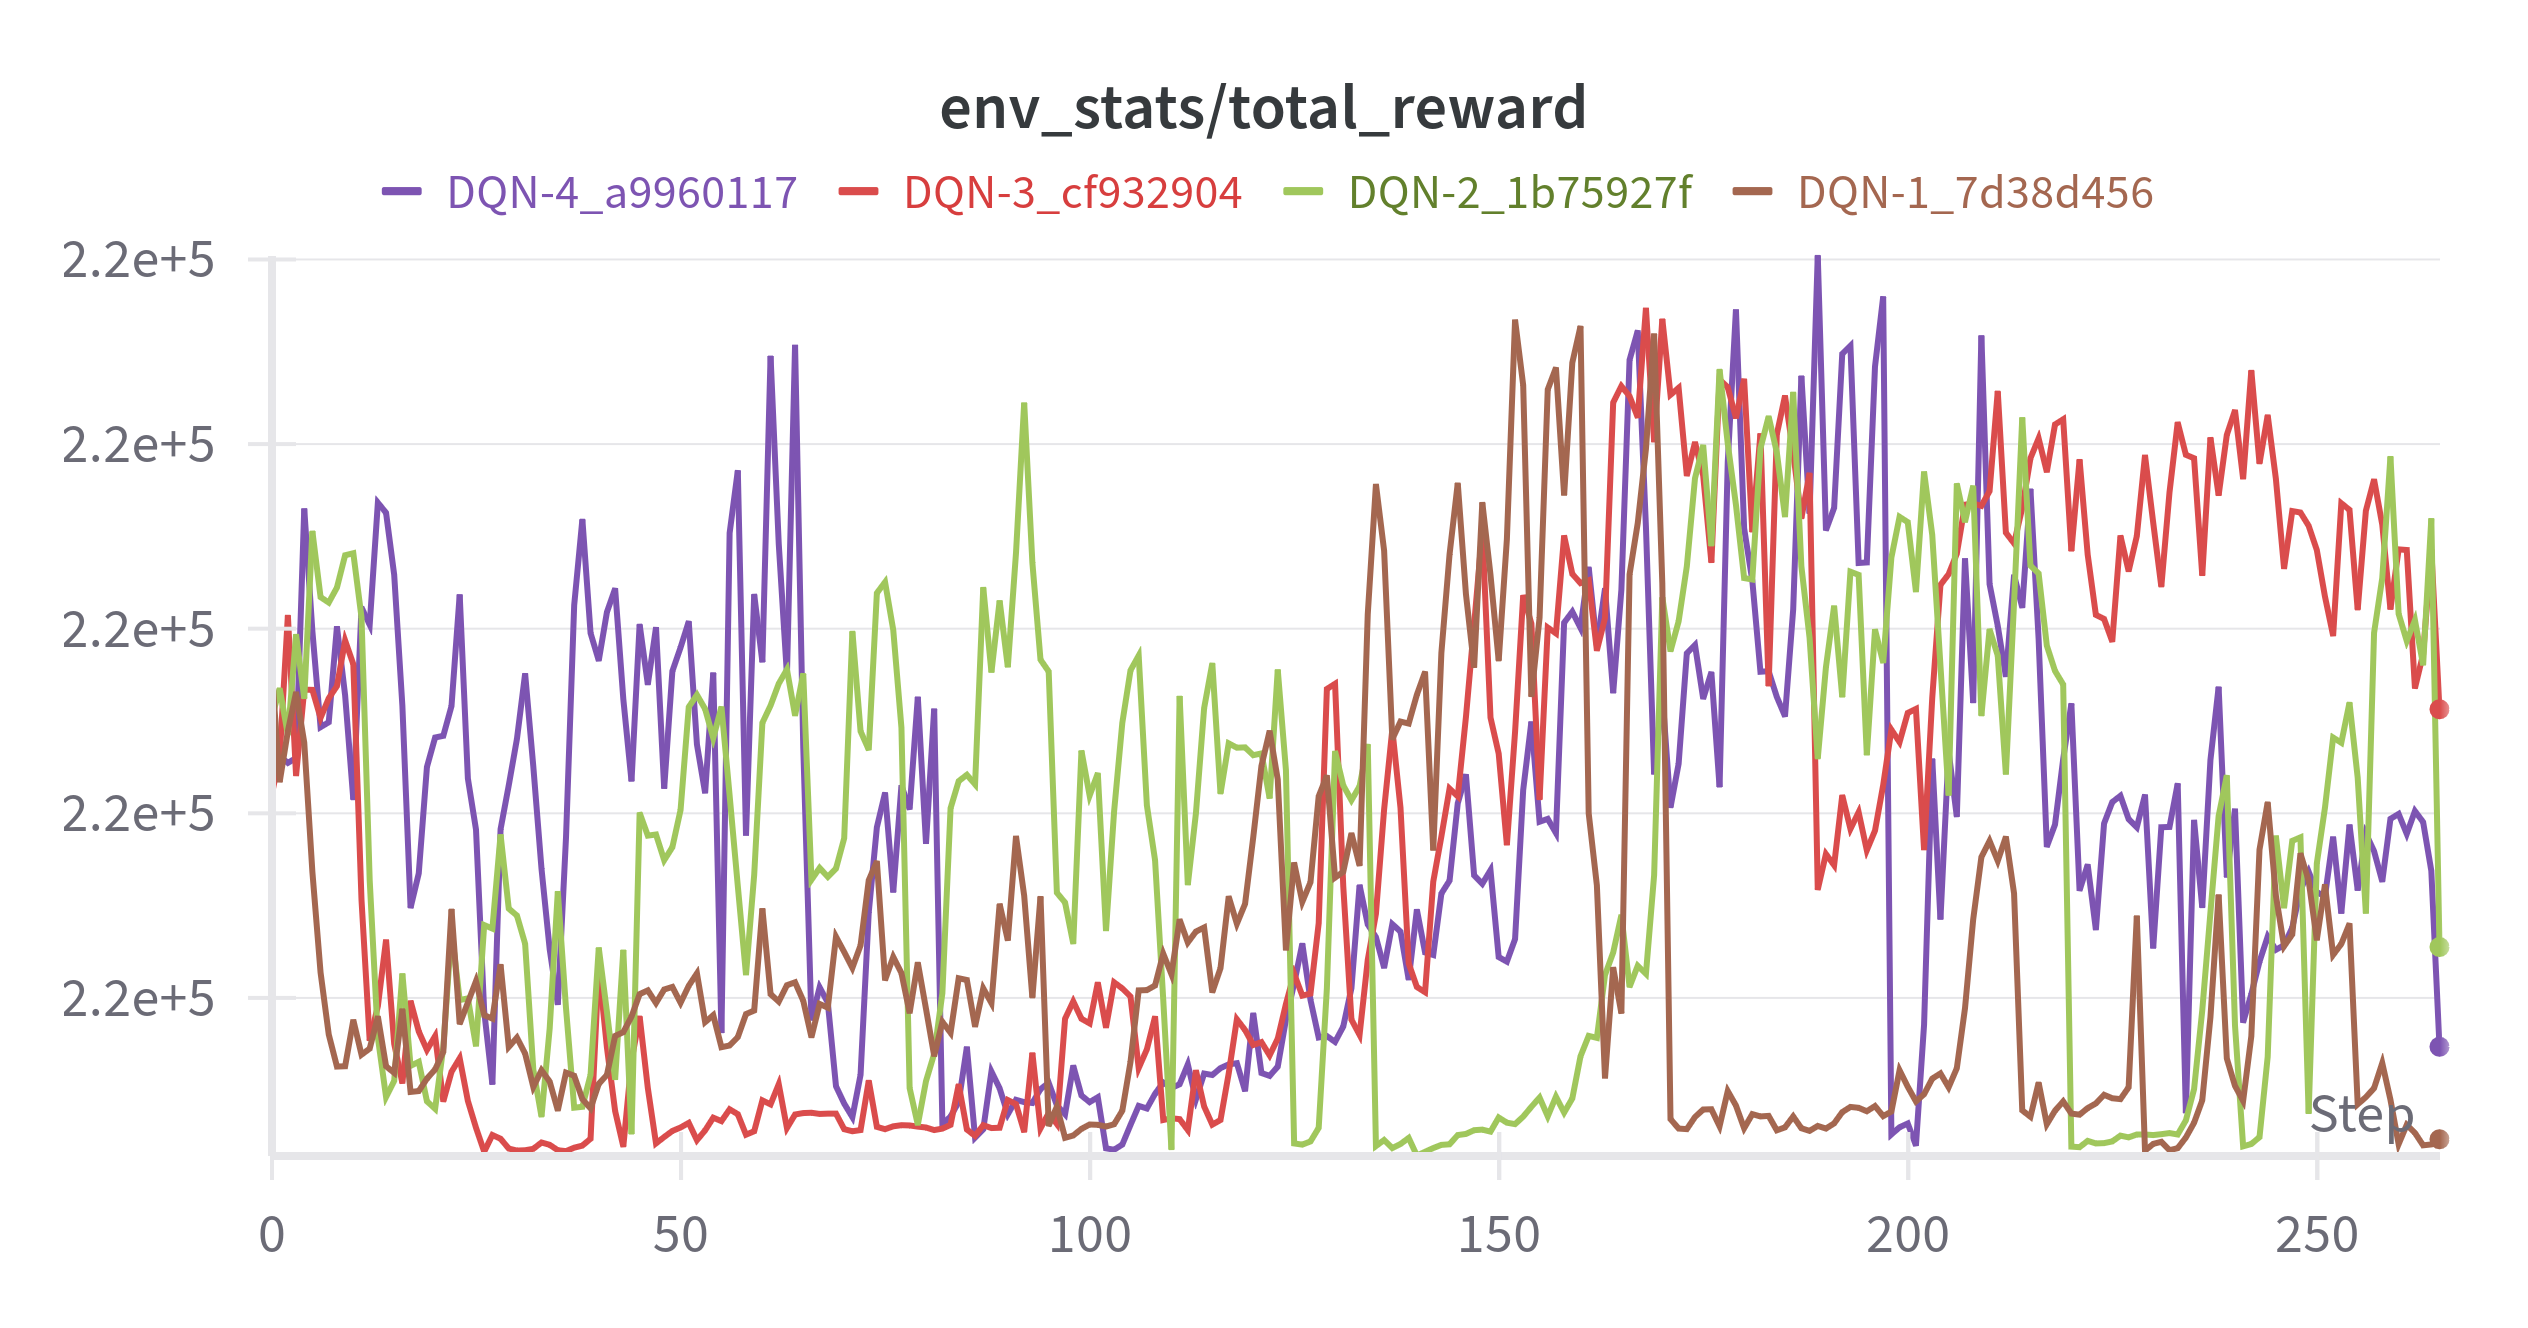
\includegraphics[width=0.8\textwidth]{figures/DQN_TotalReward.png}
    \caption{Total Reward of All DQN Agents}
    \label{fig:agent_eval_all_dqn}
\end{figure}

Figure \ref{fig:agent_eval_all_dqn} shows the performance of all 4 DQN agents of total\_reward against episode. The figure shows all 4 performing agents did not show signs of reaching the optimal policy as the total reward did not reach a plateau nor did the total reward show a dramatic difference from the start of training to the end of training. Moreover, the graph displays the average total reward of 10 episodes, which is why the x-axis is not in steps or go up till the 2,667 episodes that the agents were trained for.

\begin{figure}[H]
    \centering
    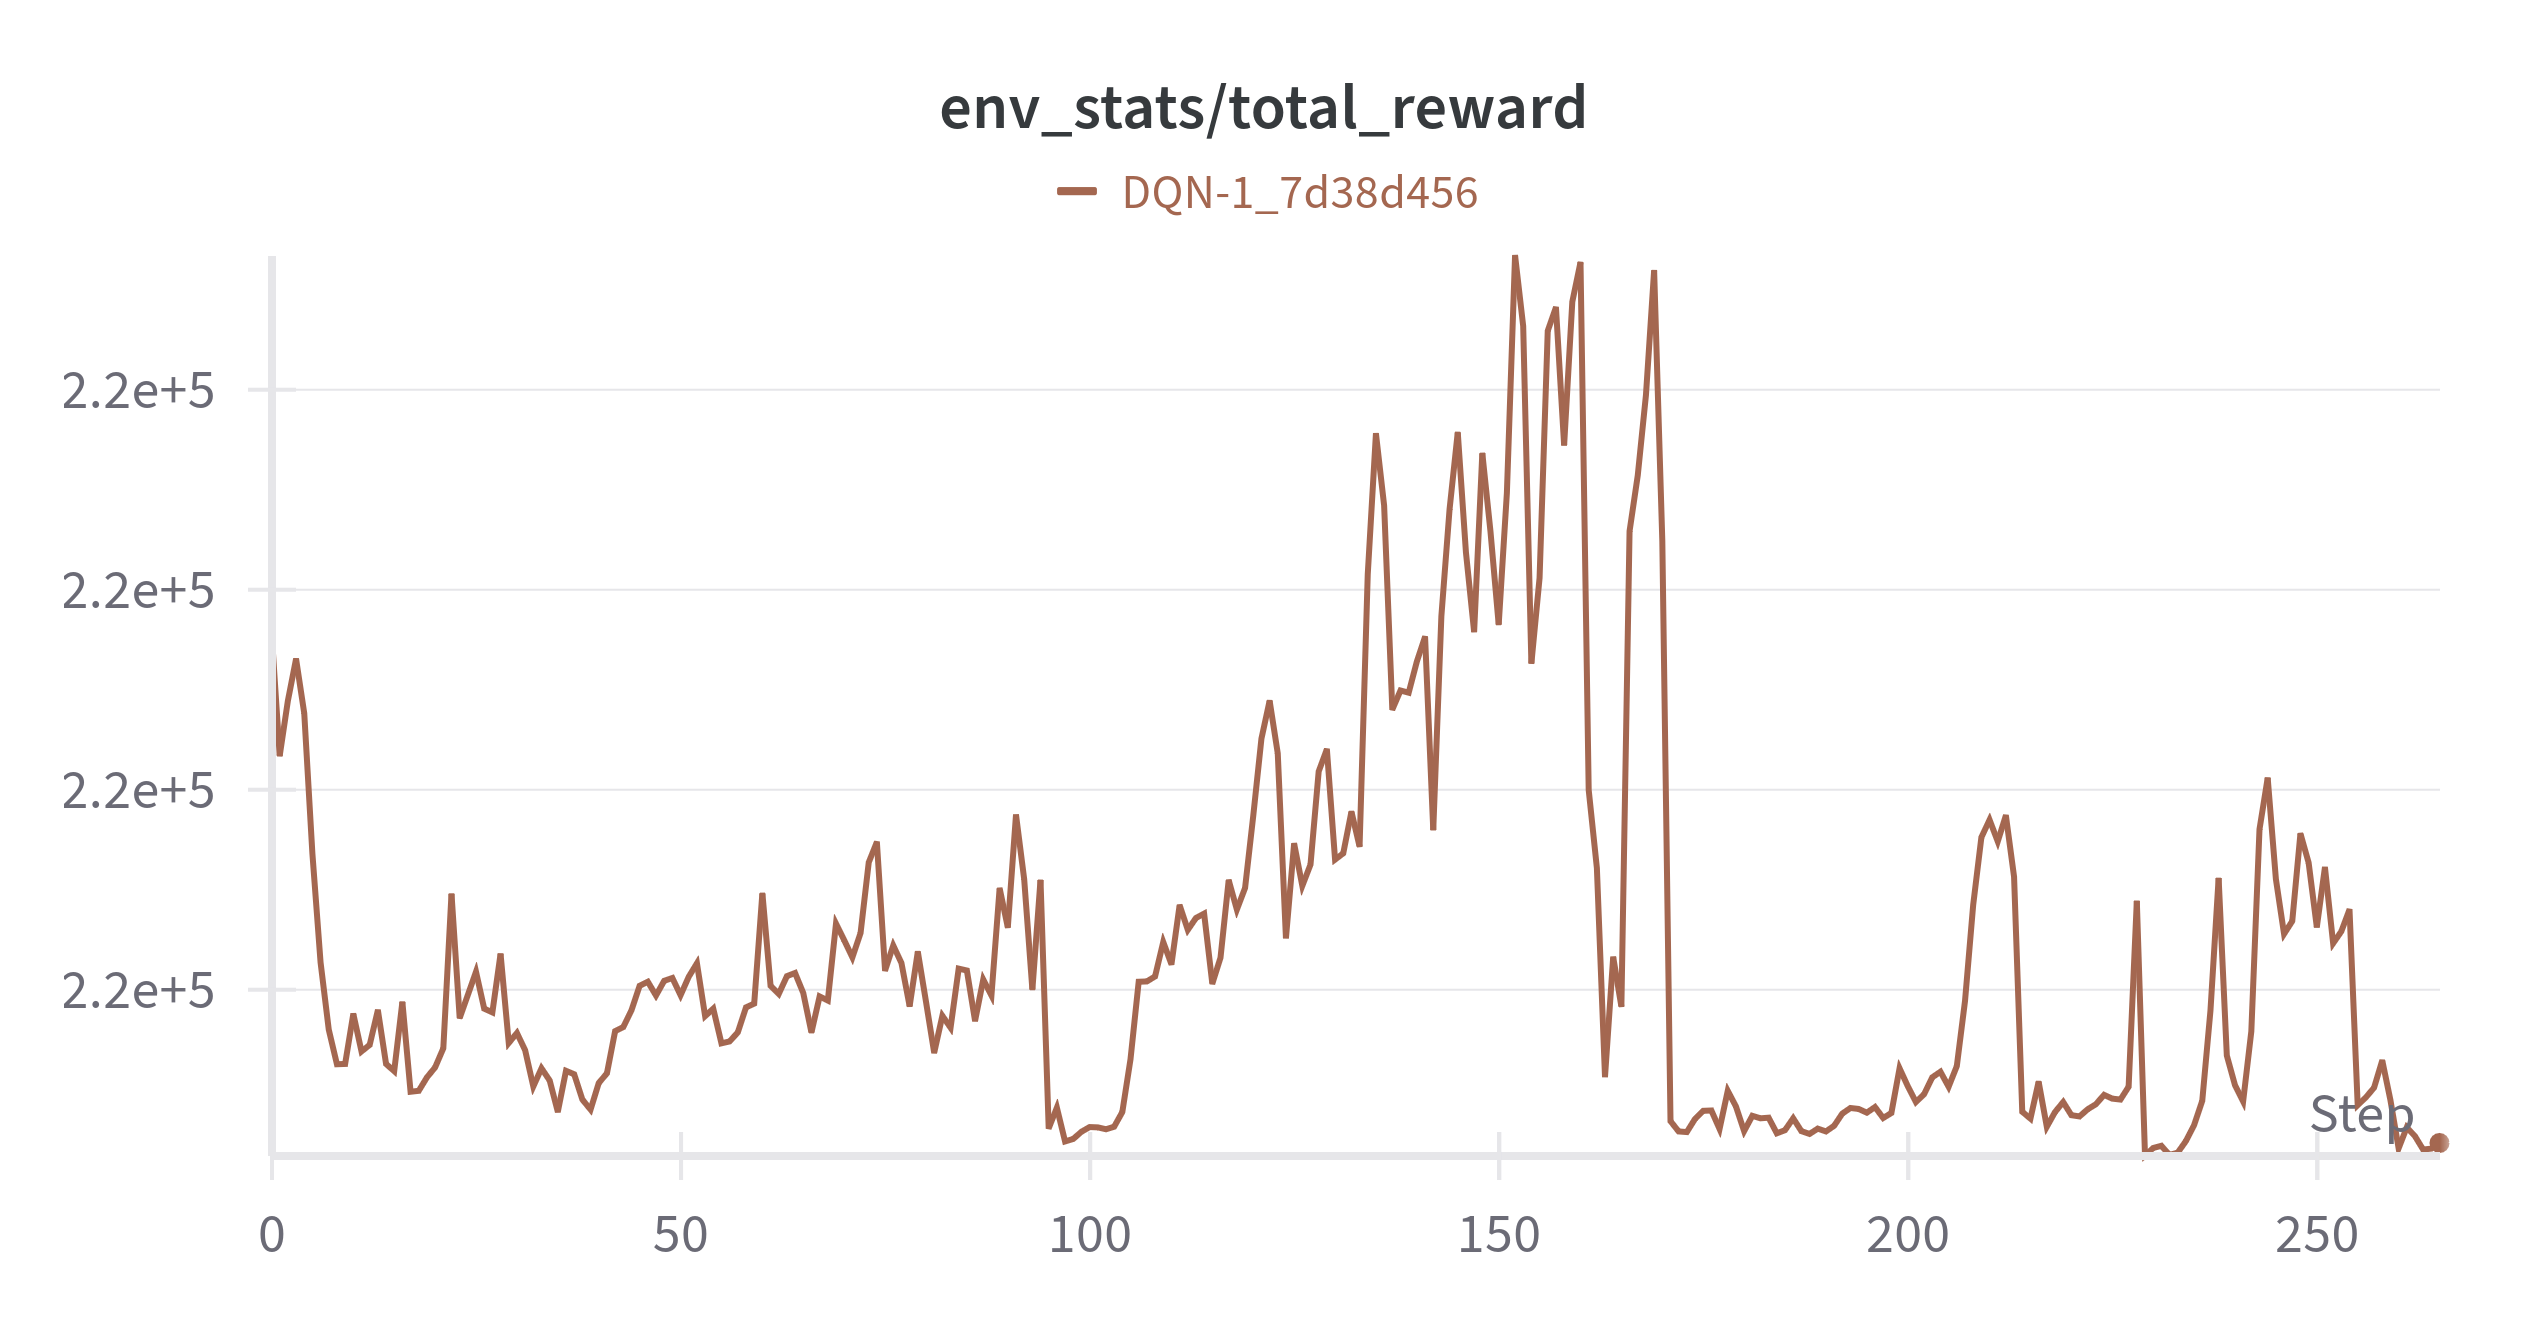
\includegraphics[width=0.7\textwidth]{figures/DQN-1_TotalReward.png}
    \caption{Total Reward of DQN Agent 1}
    \label{fig:agent_eval_dqn_1}
\end{figure}

Figure \ref{fig:agent_eval_dqn_1} shows the performance of the first DQN agent of total\_reward against episode. The figure shows that the agent did not show signs of reaching the optimal policy as the performance of the agent peaked at around 150 episodes followed by a sharp fall in performance. This suggests that the agent was still exploring the environment and was not ready to start exploiting the environment using its already known information, as the sharp fall in performance was below the starting performance of the agent.

\begin{figure}[H]
    \centering
    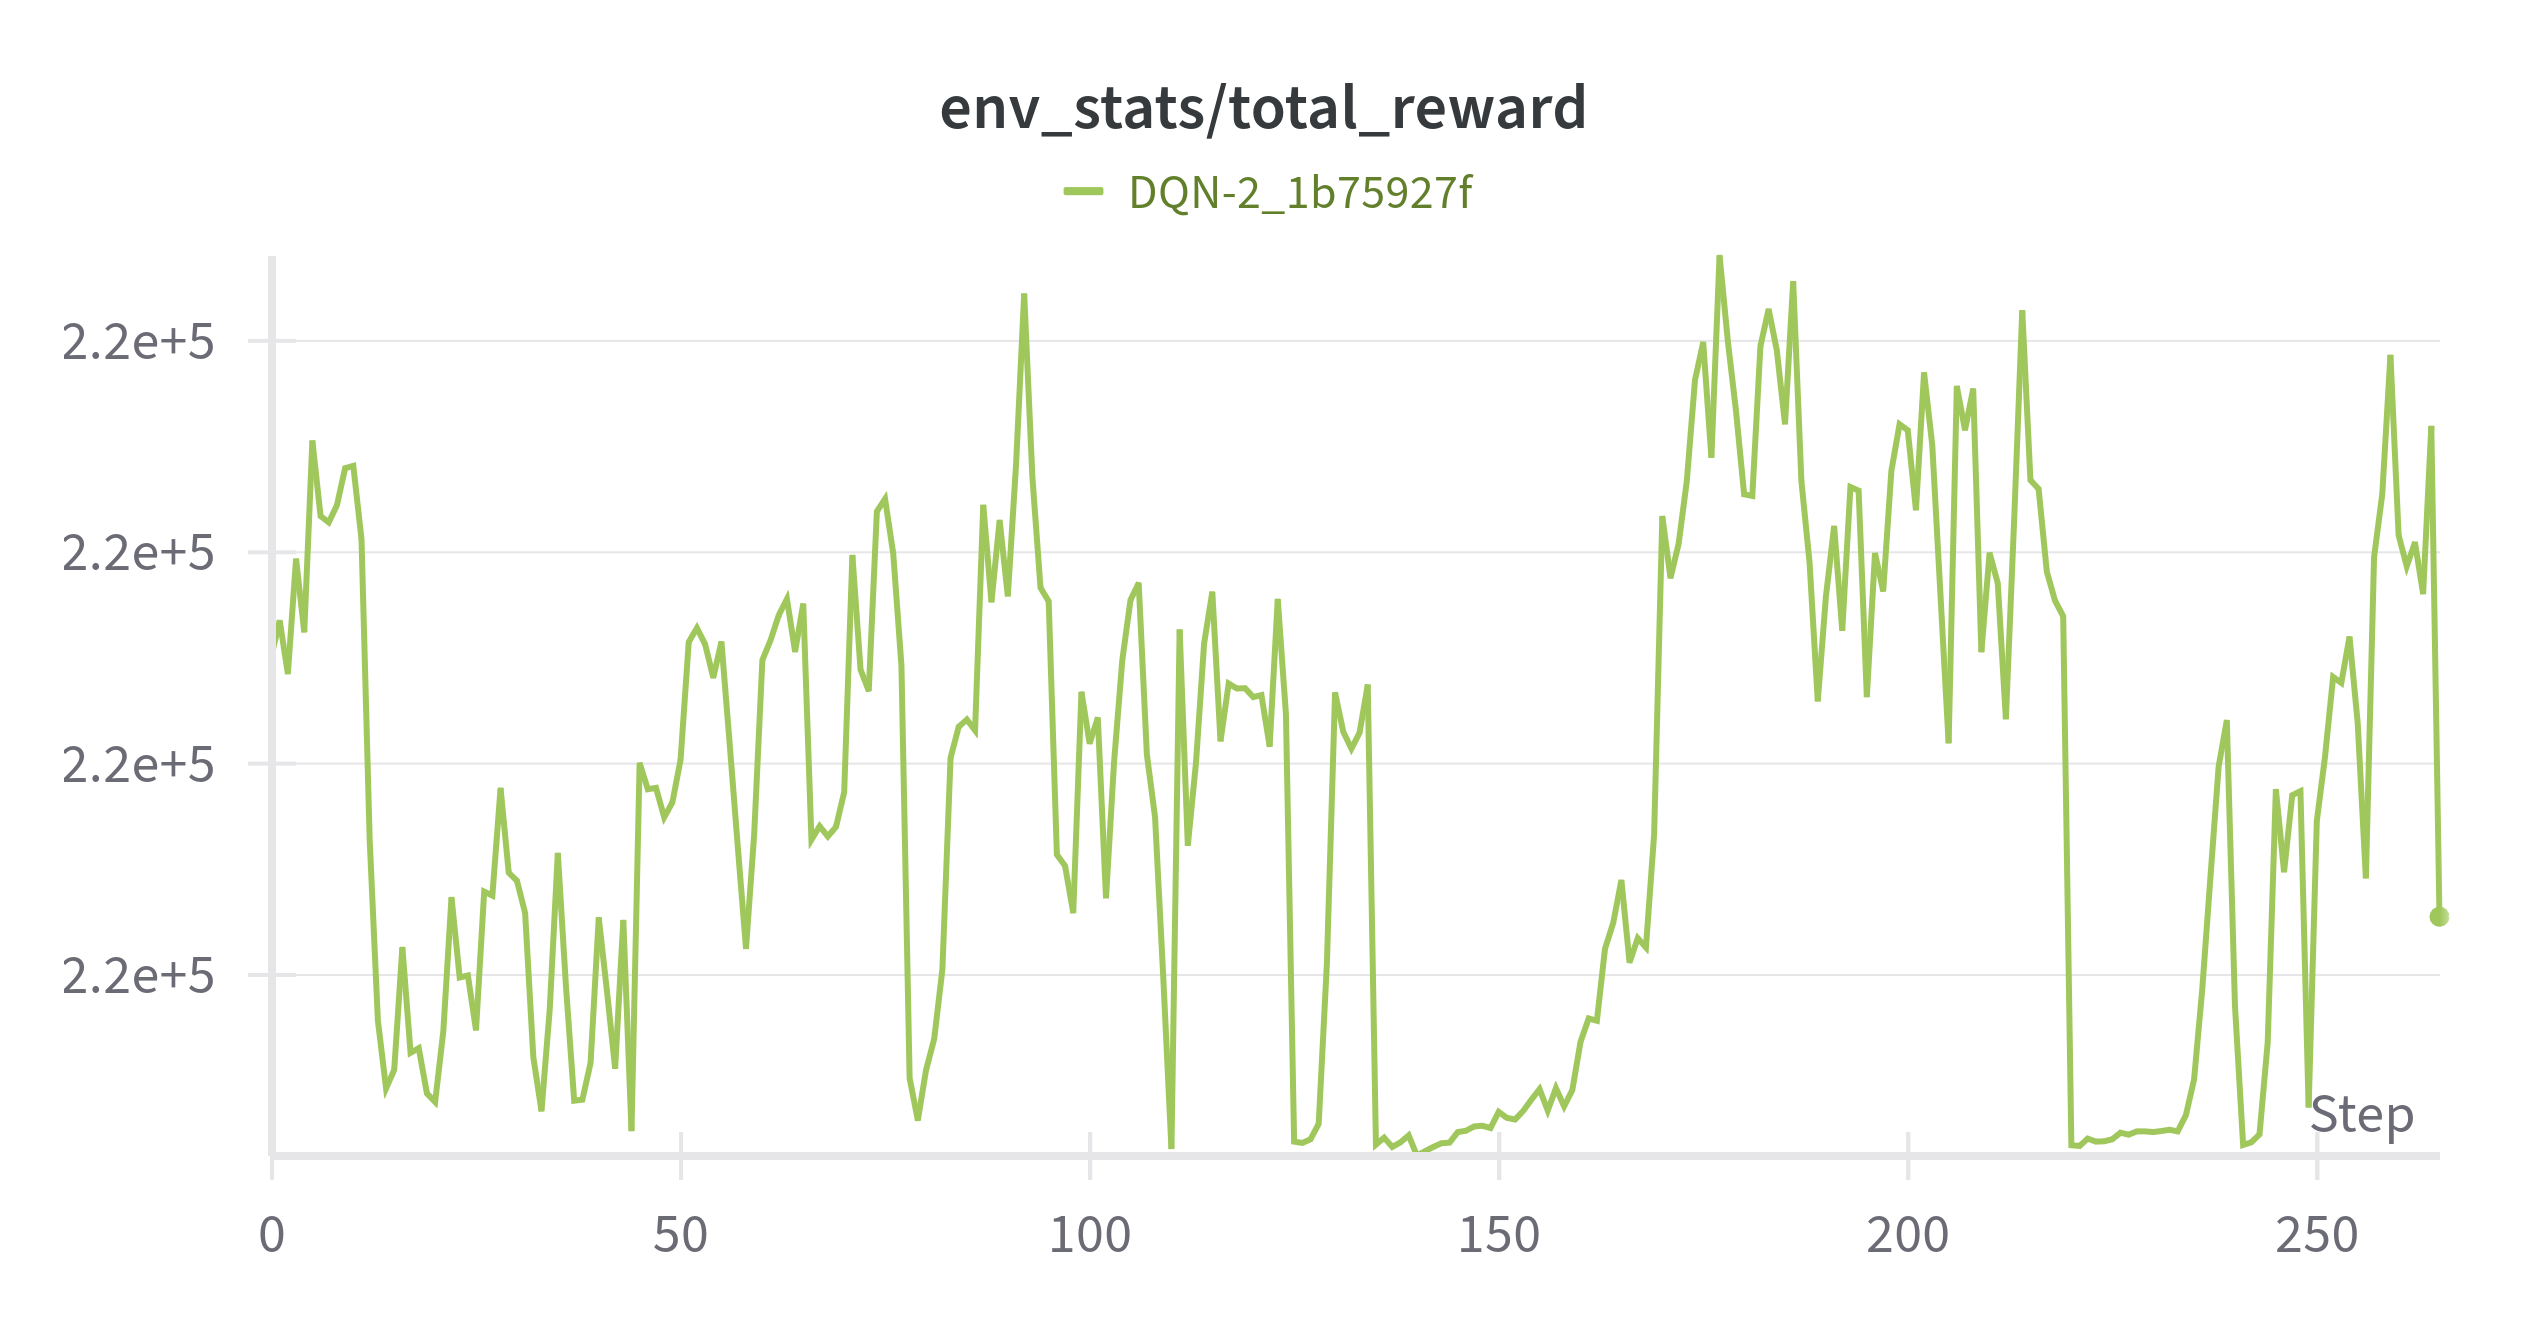
\includegraphics[width=0.7\textwidth]{figures/DQN-2_TotalReward.png}
    \caption{Total Reward of DQN Agent 2}
    \label{fig:agent_eval_dqn_2}
\end{figure}

Figure \ref{fig:agent_eval_dqn_2} shows the performance of the second DQN agent of total\_reward against episode. The figure shows that the agent did show signs of significant amount of exploration, as there was a range of episodes where the agent had high and low performance. This suggests that the agent was still exploring the environment. However, the agent did have a consistently high amount of performance between episodes 170 and 210.

\begin{figure}[H]
    \centering
    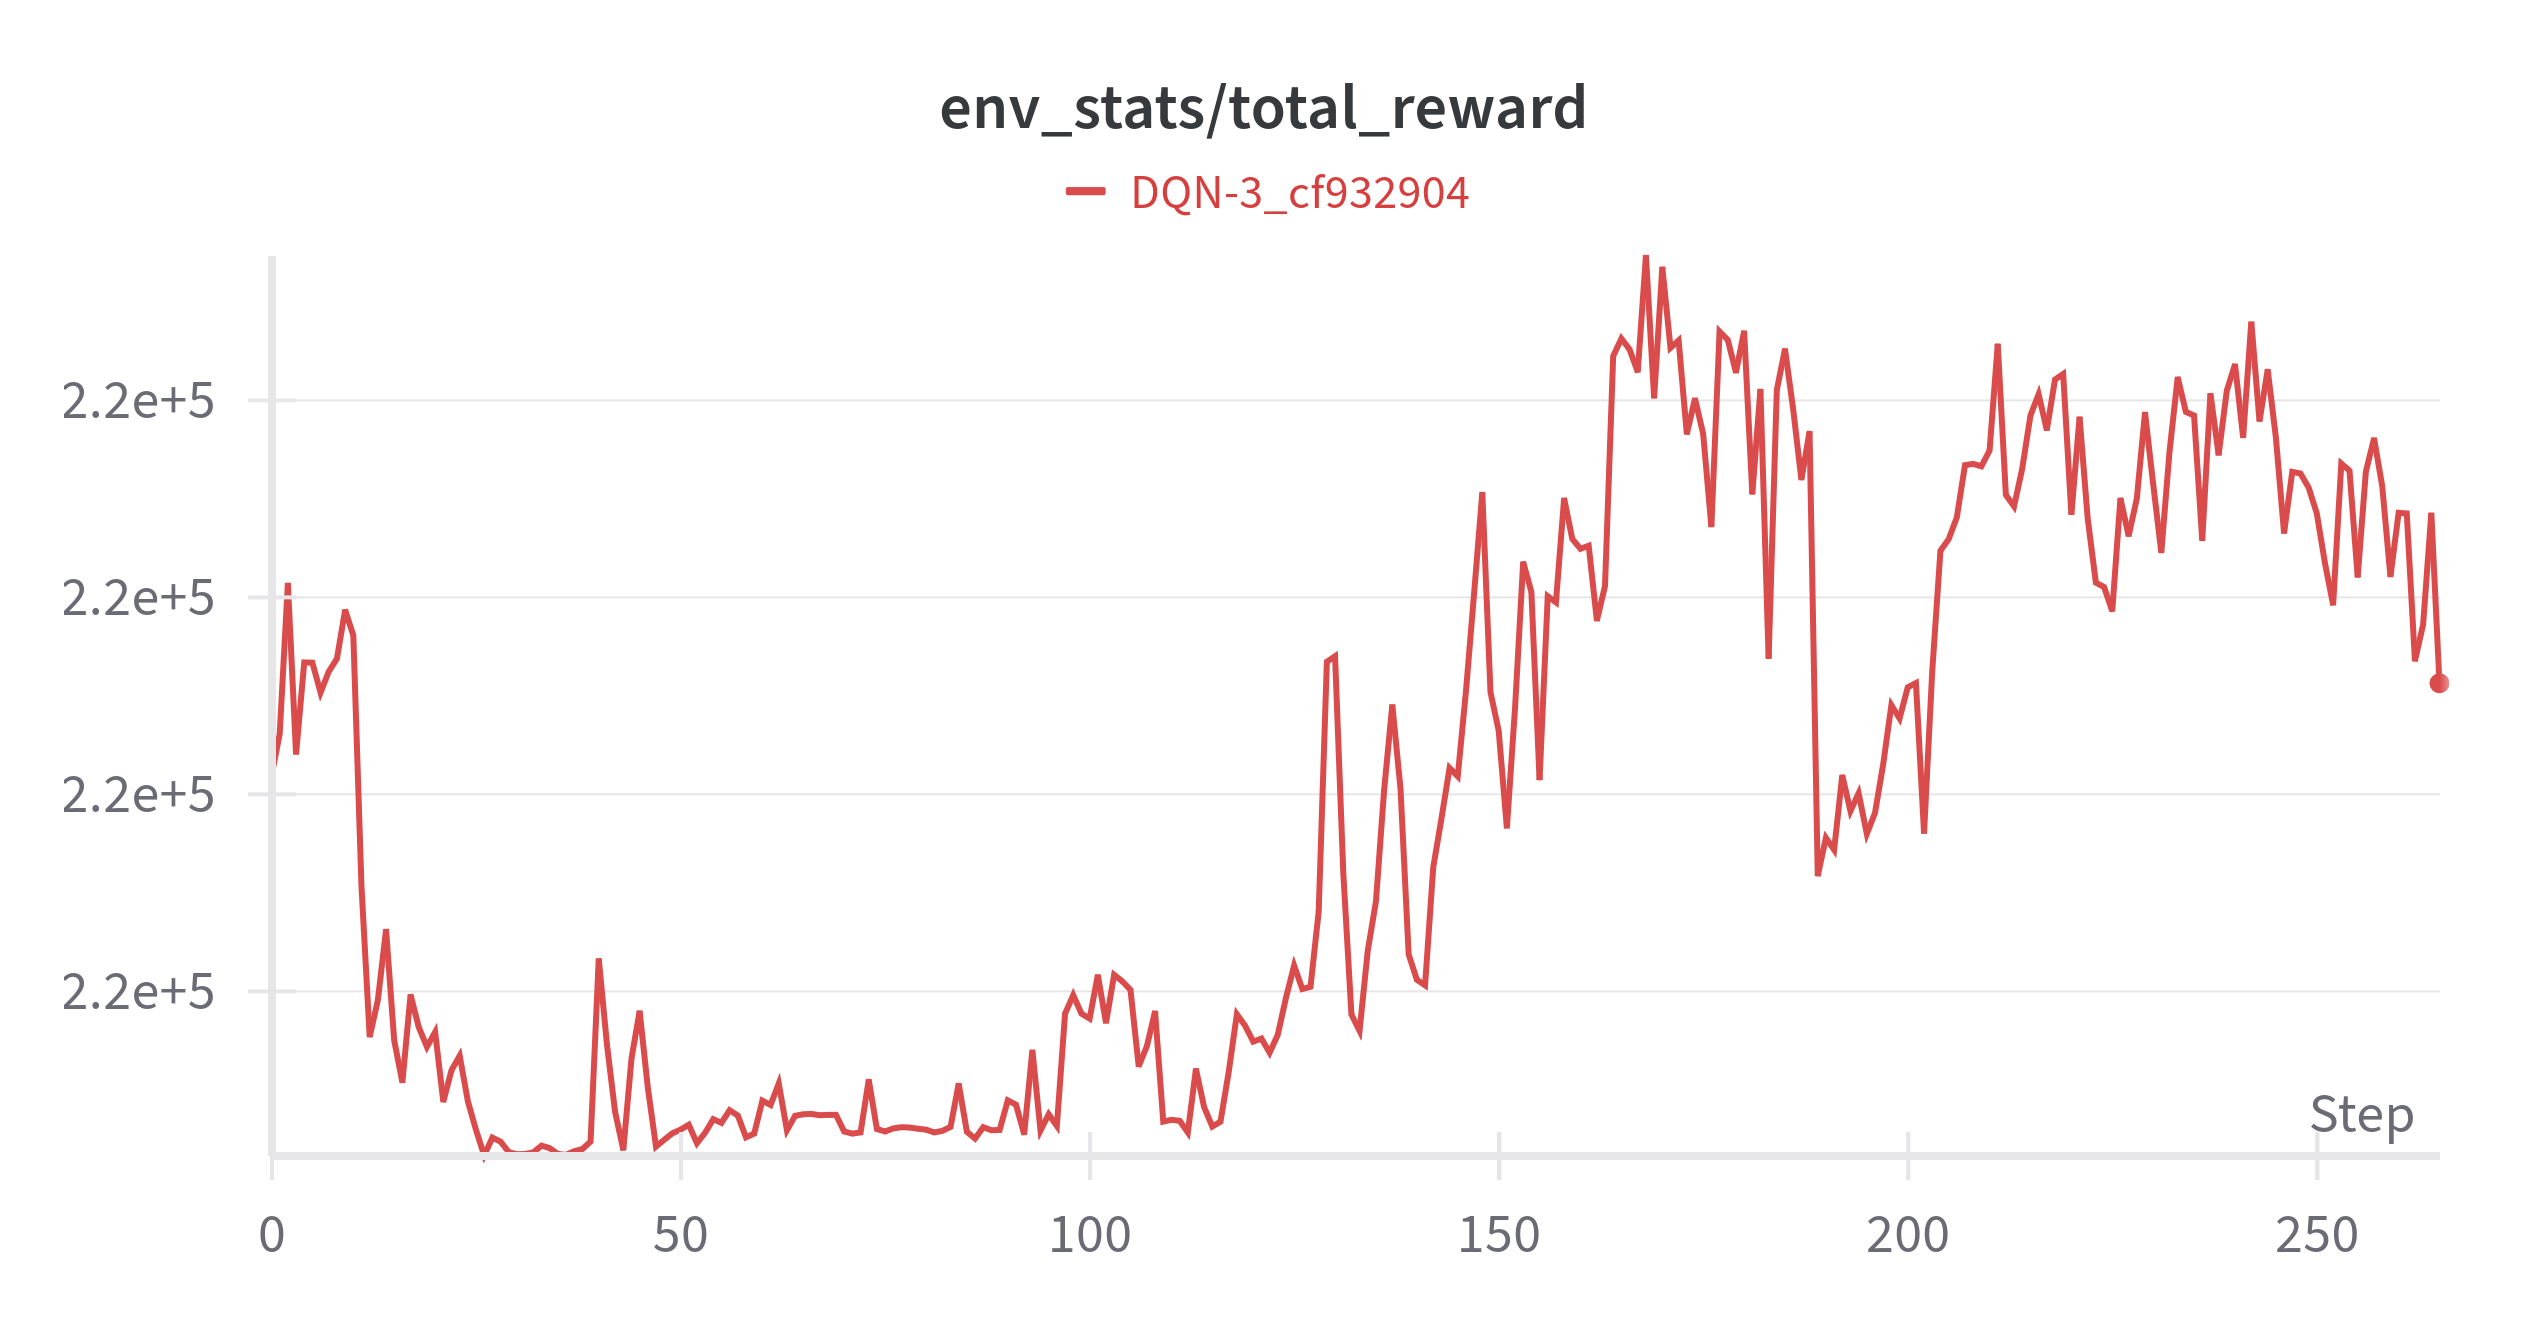
\includegraphics[width=0.7\textwidth]{figures/DQN-3_TotalReward.png}
    \caption{Total Reward of DQN Agent 3}
    \label{fig:agent_eval_dqn_3}
\end{figure}

Figure \ref{fig:agent_eval_dqn_3} shows the performance of the third DQN agent of total\_reward against episode. The figure shows that the agent did show signs of exploration, as the training of the agent started with a low amount of performance and gradually increased in performance between episode 10 and 150. This suggests that the agent was able to slowly learn the environment that was trained on and shows signs of gradual learning. Moreover, the agent was able to reach a peak performance at around episode 150 and is the best performing agent out of the DQN agents so far due to its consistently high performance. 

\begin{figure}[H]
    \centering
    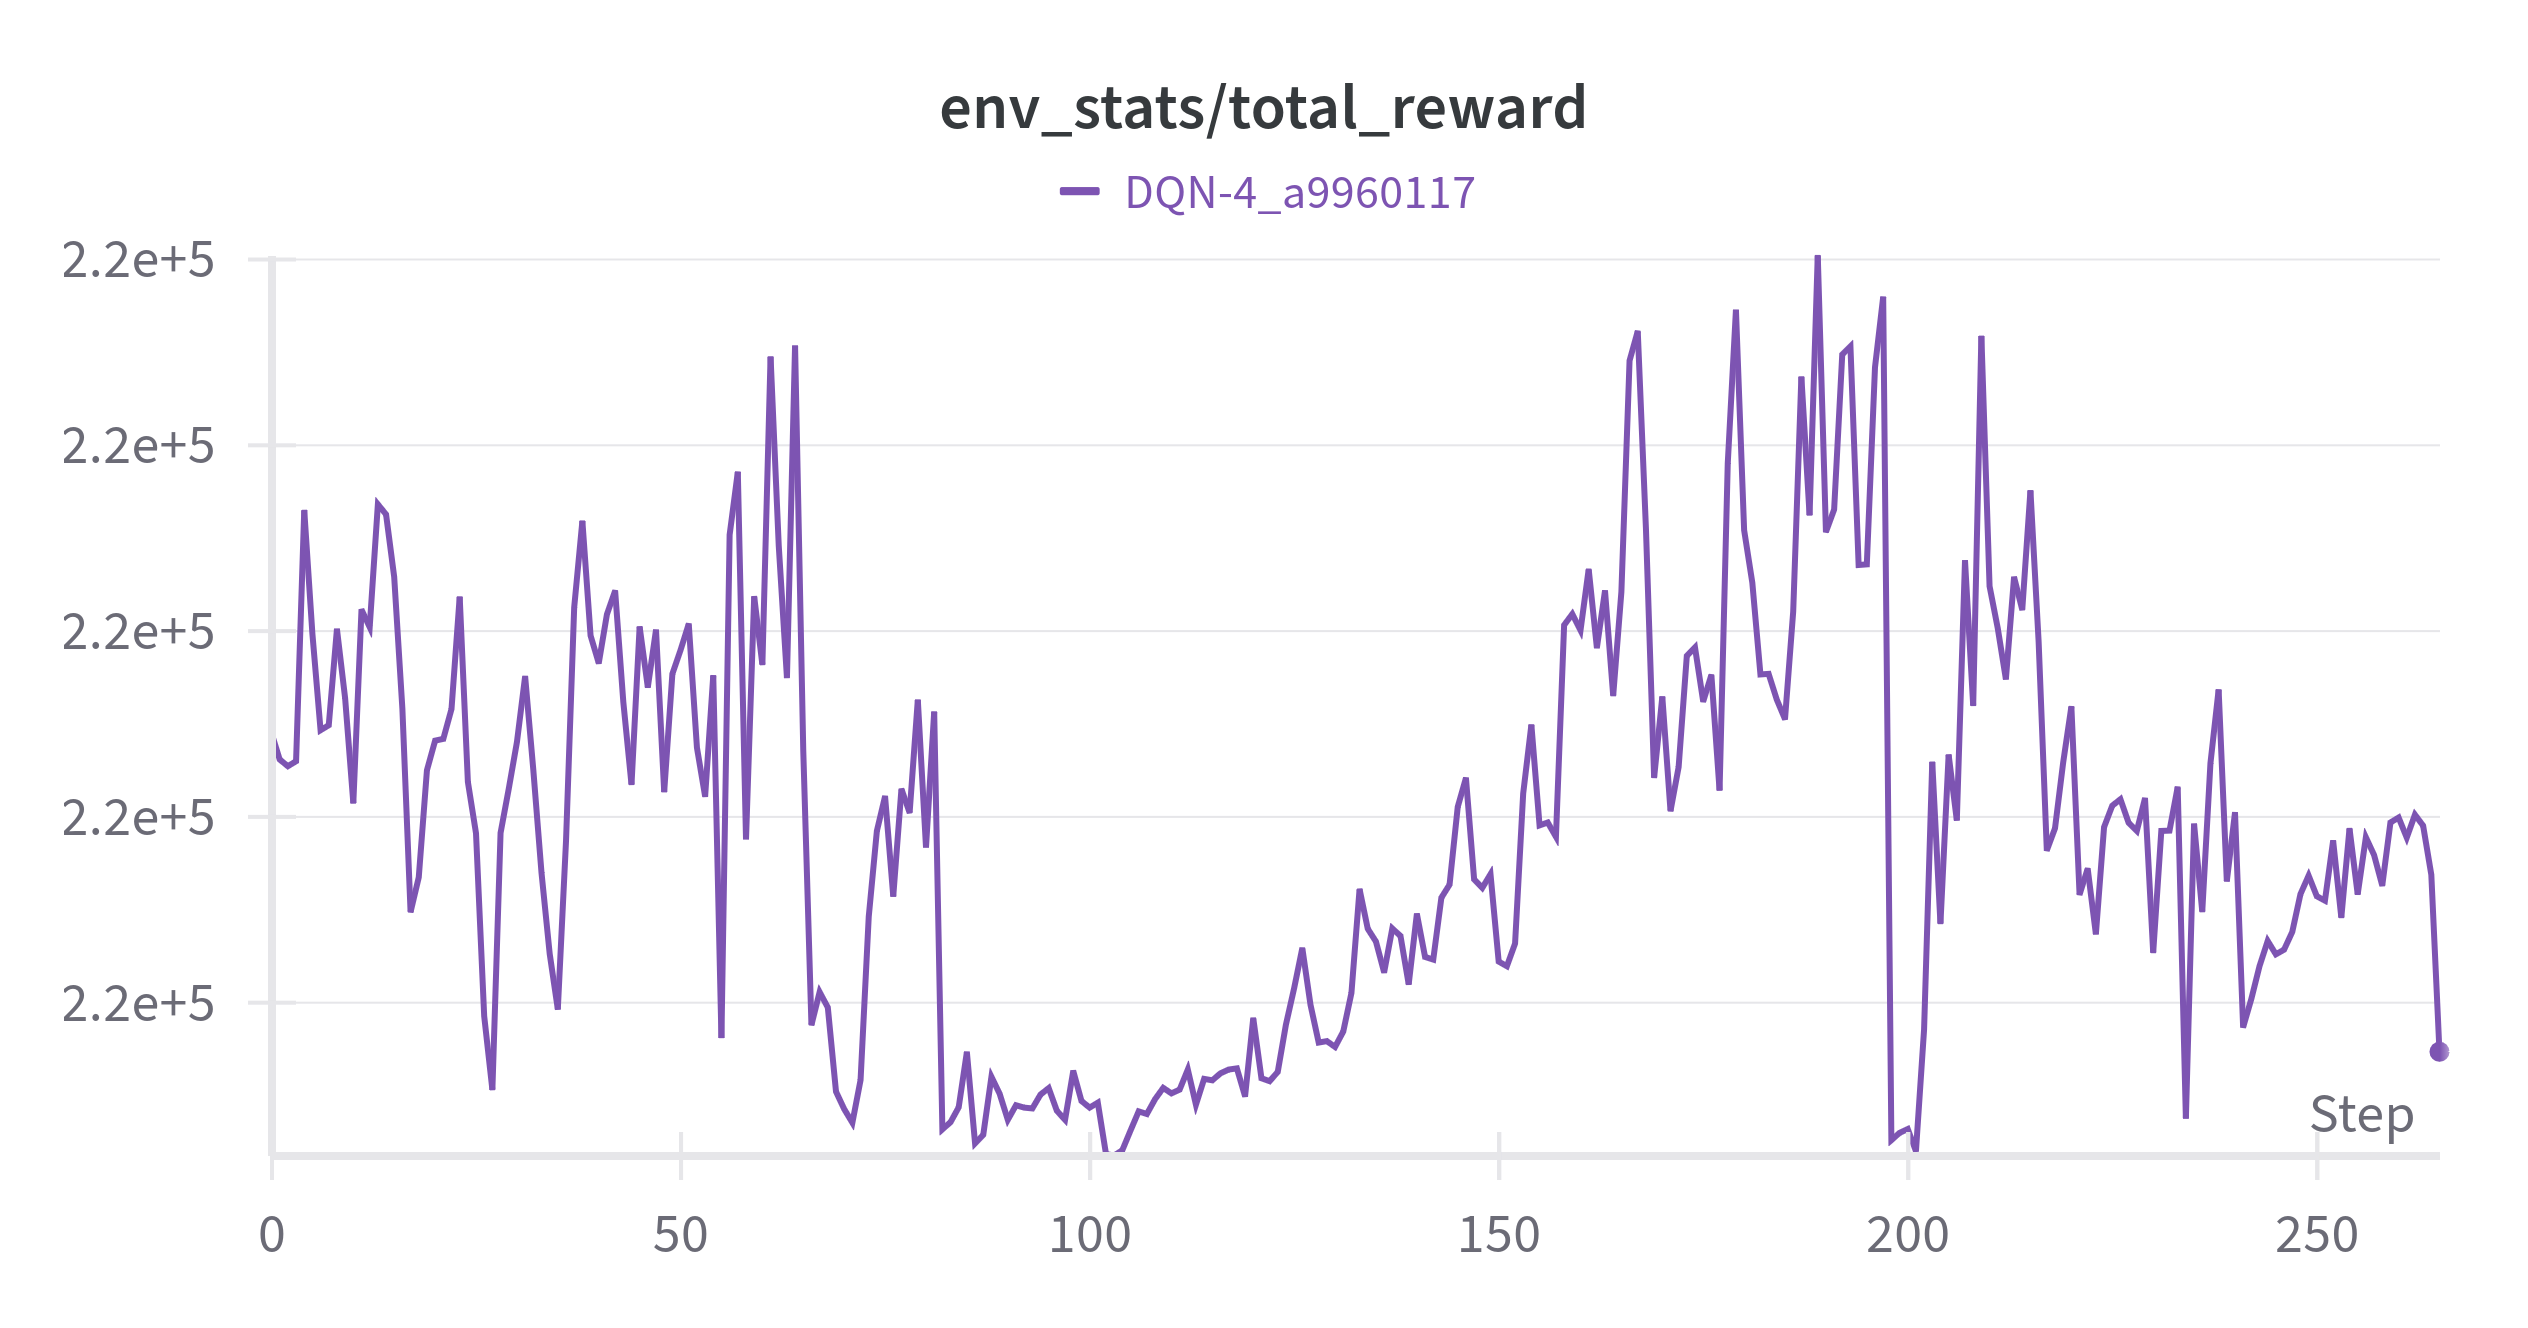
\includegraphics[width=0.7\textwidth]{figures/DQN-4_TotalReward.png}
    \caption{Total Reward of DQN Agent 4}
    \label{fig:agent_eval_dqn_4}
\end{figure}

Figure \ref{fig:agent_eval_dqn_4} shows the performance of the fourth DQN agent of total\_reward against episode. The figure shows that the agent shows weak signs of an understanding of the environment due to its low performance throughout the training. The agent did not show any signs of consistently high performance as drops in performance always followed high peaks. This highly suggests that the agent was still exploring the environment and never reached a point where it was able to exploit the environment using its already known information.

In conclusion, the best performing DQN agent from the list of 4 agents is agent 3 because of its consistently high performance throughout the training. The agent was able to learn the environment and exploit the environment using its already known information, which is evident from the inital low amount of reward followed by a strong growth in average reward. This further suggests that the agent shows signs of being able to go through cycles of learning and exploiting before reaching the optimal policy. 

\subsection{QR-DQN}

The training script used to train all 4 agents can be found within the research paper's GitHub repository under ``run\_baseline\_QRDQN.py''. A total of 8 parallel instances of the environment was trained at the same time to train for 3,333 episodes total, where each episode is 1,500 steps long. This totals up to 39,996,000 steps in total. The performance of the 4 agents can be seen on figure \ref{fig:agent_eval_all_qrdqn} . 

\begin{figure}[H]
    \centering
    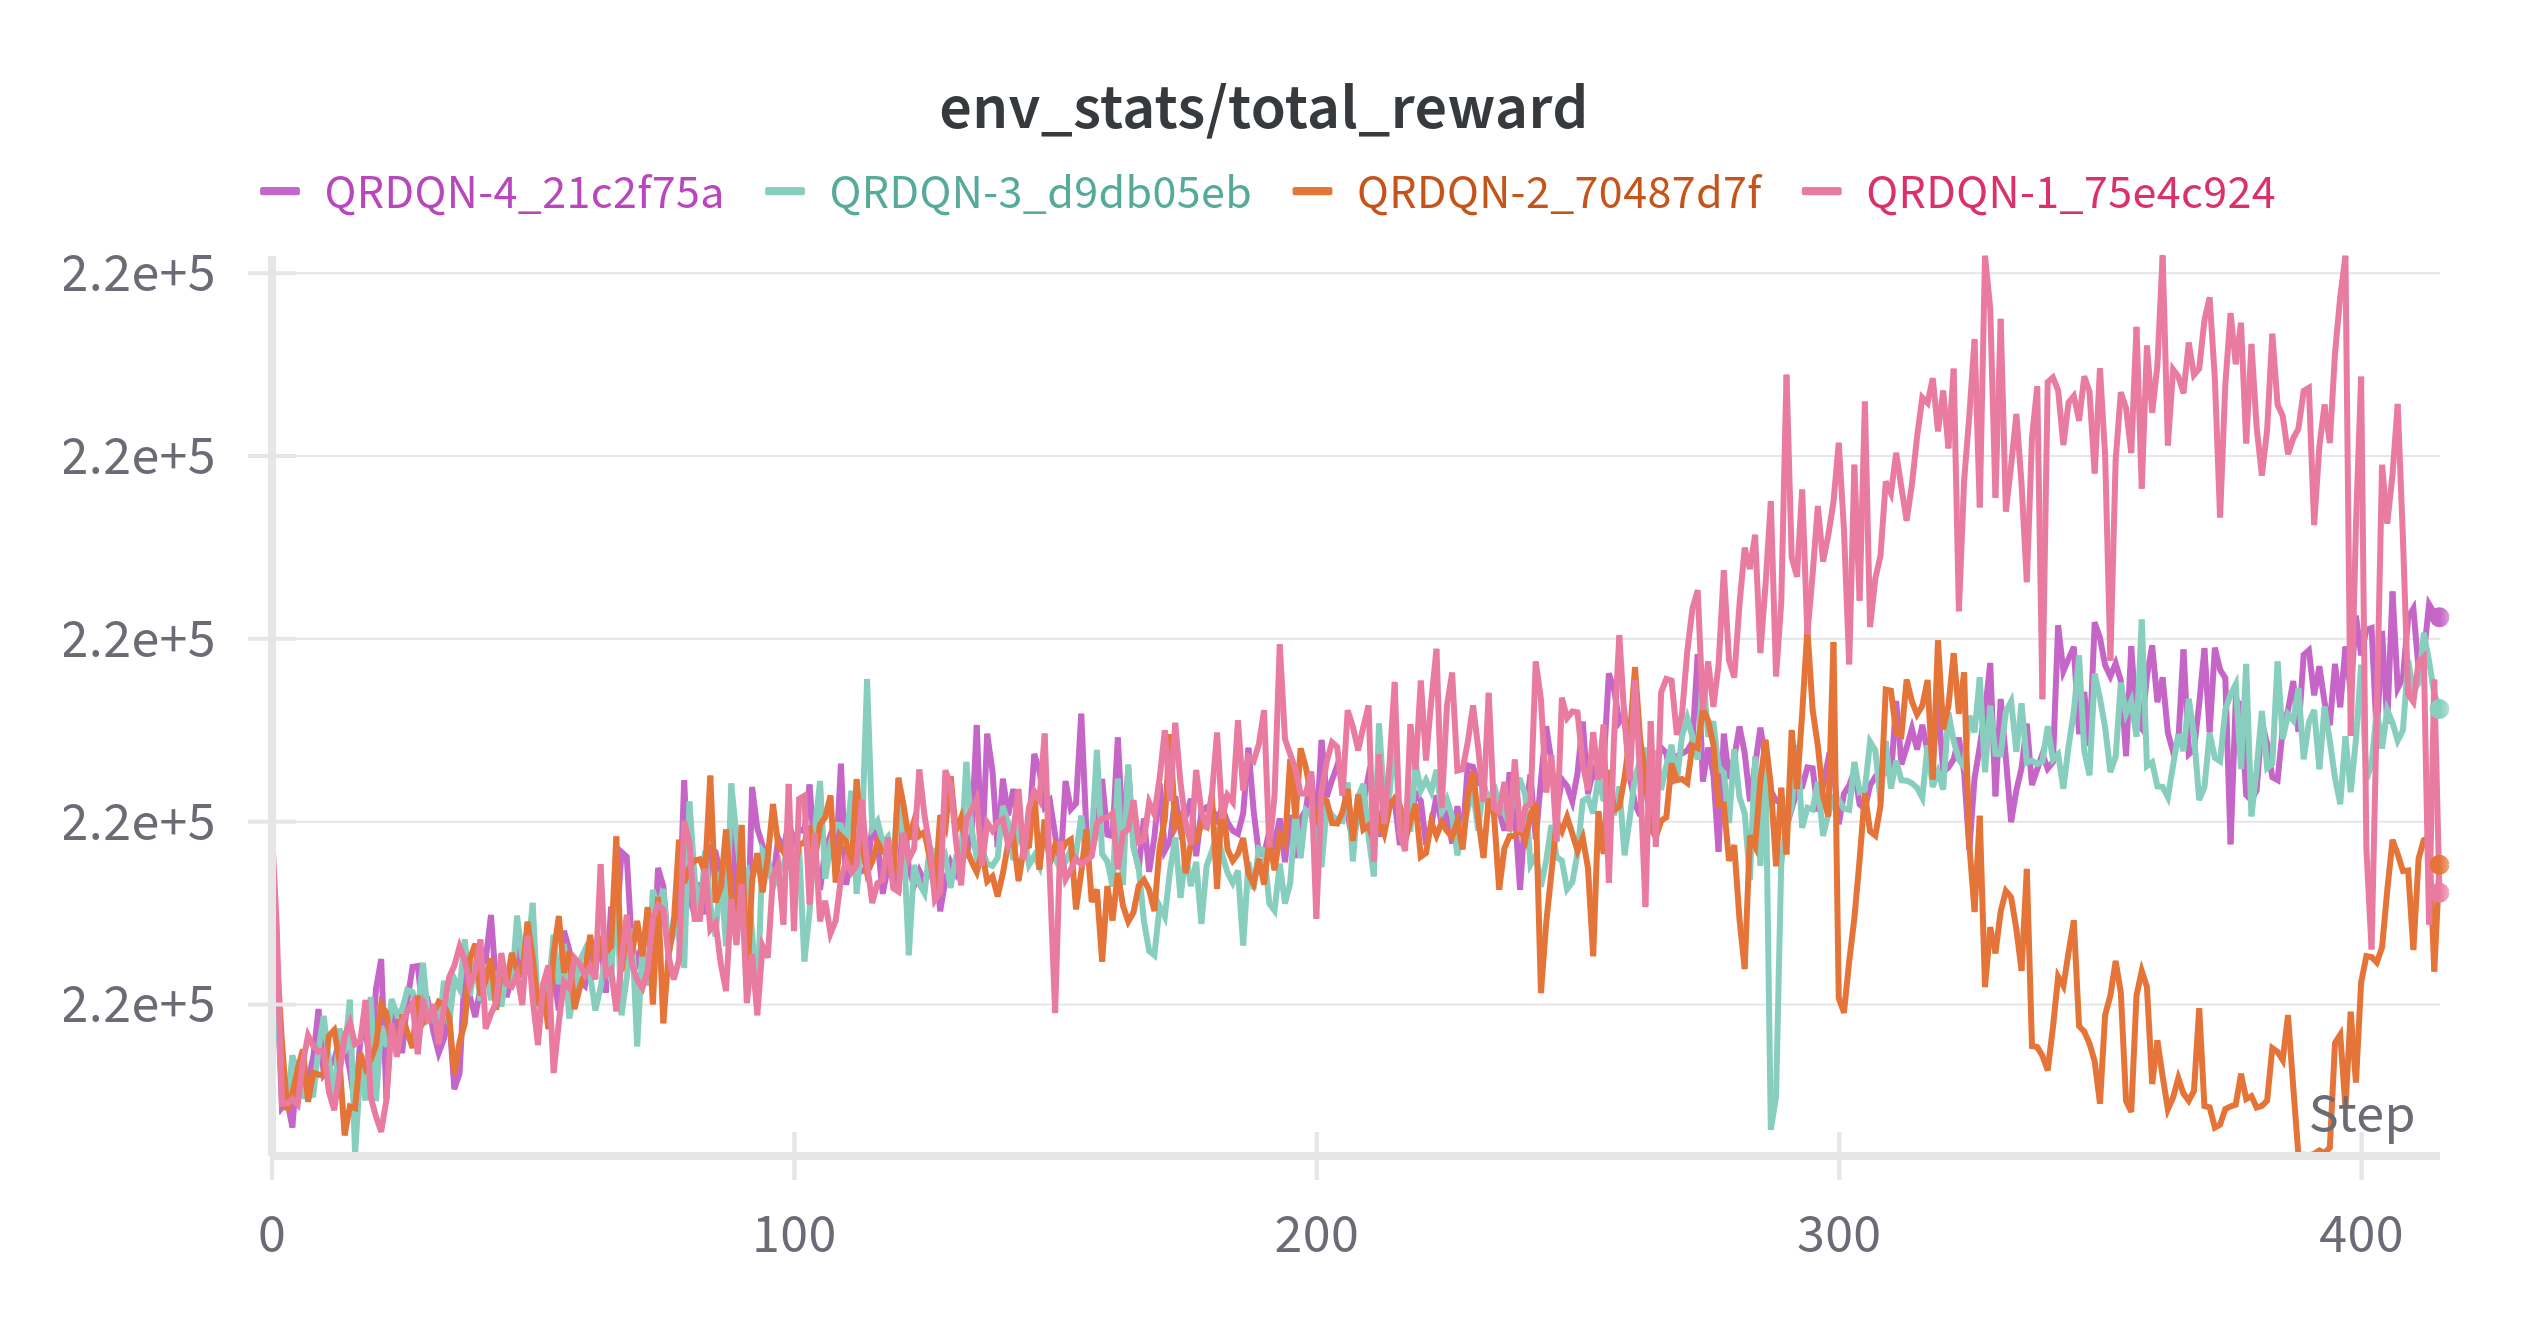
\includegraphics[width=0.8\textwidth]{figures/QRDQN_TotalReward.png}
    \caption{Total Reward of All QRDQN Agents}
    \label{fig:agent_eval_all_qrdqn}
\end{figure}

Compared to the DQN agents, the QR-DQN agents show a more promising performance in terms of total reward. The figure above shows the performance of all 4 QR-DQN agents of total\_reward against episode and shows that all 4 agents had a very similar but consistent growth in performance. Between episodes 0 and 200, all 4 agents had a similar amount of performance, but after episode 200, the agents started to diverge. QRDQN agent 3 and 4 had similar amounts of performance, where both agents had a very flat but consistently positive amount of growth. QRDQN agent 2 had a dramatic fall in performance from episode 270 to 370, but was able to swiftly recover and reach a peak performance at episode 400 but not enough data is available to determine if the agent would consistently kept this level of performance. QRDQN agent 1 spiked in performance and was able to maintain a high level of performance throughout the training, despite the sharp but short falls in performance every 50 episodes between episode 300 and 400. 

Despite the graph implying that QRDQN agent 1 is the best performing agent, only looking at the average total reward is not enough to come to this conclusion. Therefore, the graph below showing the average loss of each agent will be used to determine the best performing agent.

\begin{figure}[H]
    \centering
    \includegraphics[width=0.8\textwidth]{figures/QRDQN_Loss.png}
    \caption{Loss of All QRDQN Agents}
    \label{fig:agent_eval_all_qrdqn_loss}
\end{figure}

Figure \ref{fig:agent_eval_all_qrdqn_loss} showing the training loss of each agent shows that all 4 agents showed consistently low loss values with QRDQN agent 1 and 4 having large spikes of loss values of 8 and above. However, all agents had consistently low loss values with consistent random spikes, which further suggests that the best performing agent is QRDQN agent 1.

\subsection{PPO}

The training script used to train all 4 agents can be found within the research paper's GitHub repository under ``run\_baseline\_PPO.py''. A total of 14 parallel instances of the environment was trained at the same time to train for 1,905 episodes total, where each episode is 1,500 steps long. This totals up to 40,005,000 steps in total. The performance of the 4 agents can be seen in the graph below. 

\begin{figure}[H]
    \centering
    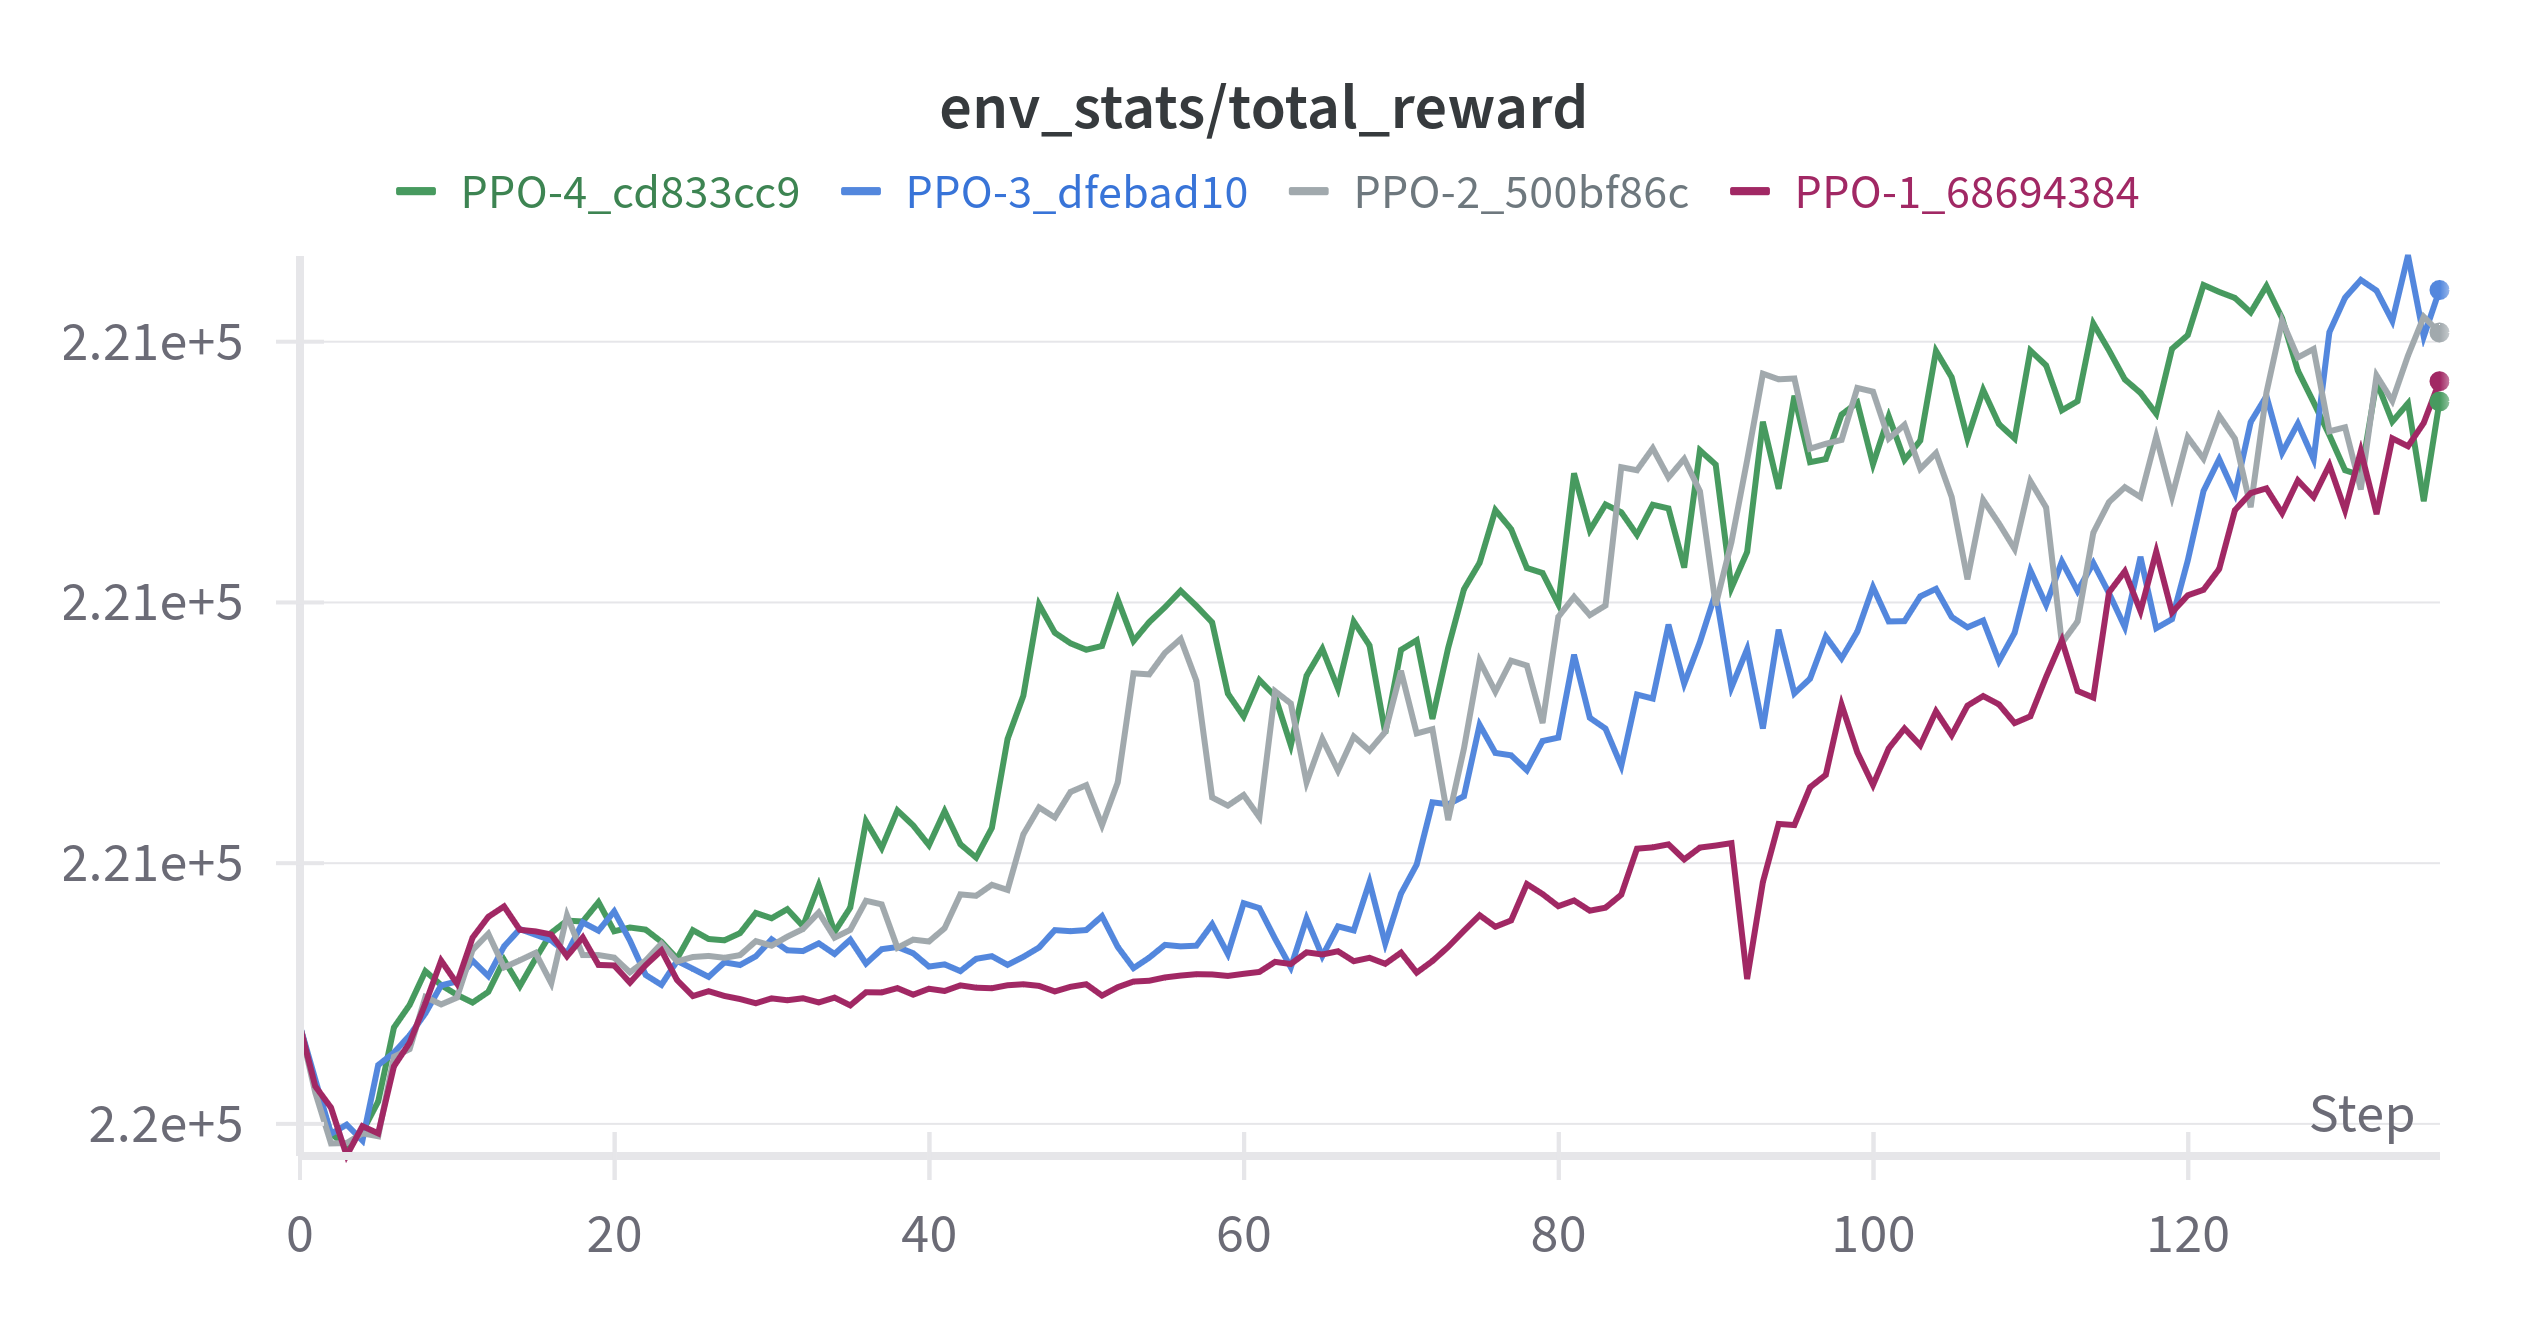
\includegraphics[width=0.8\textwidth]{figures/PPO_TotalReward.png}
    \caption{Total Reward of All PPO Agents}
    \label{fig:agent_eval_all_ppo}
\end{figure}

Looking at the performance of all 4 PPO agents, all the agents showed very strong signs of learning the environment and reaching the optimal policy. All agents maintained a gradual and strong growth in performance throughout training and all agents did not have any drops or sharp falls in total reward. Deciding the best performing agent among the 4 is difficult because all agents have very similar positive trajectories in performance. However, figure \ref{fig:agent_eval_all_ppo_loss}, below, showing the average loss of each agent will be used to find more information on the best performing agent.

\begin{figure}[H]
    \centering
    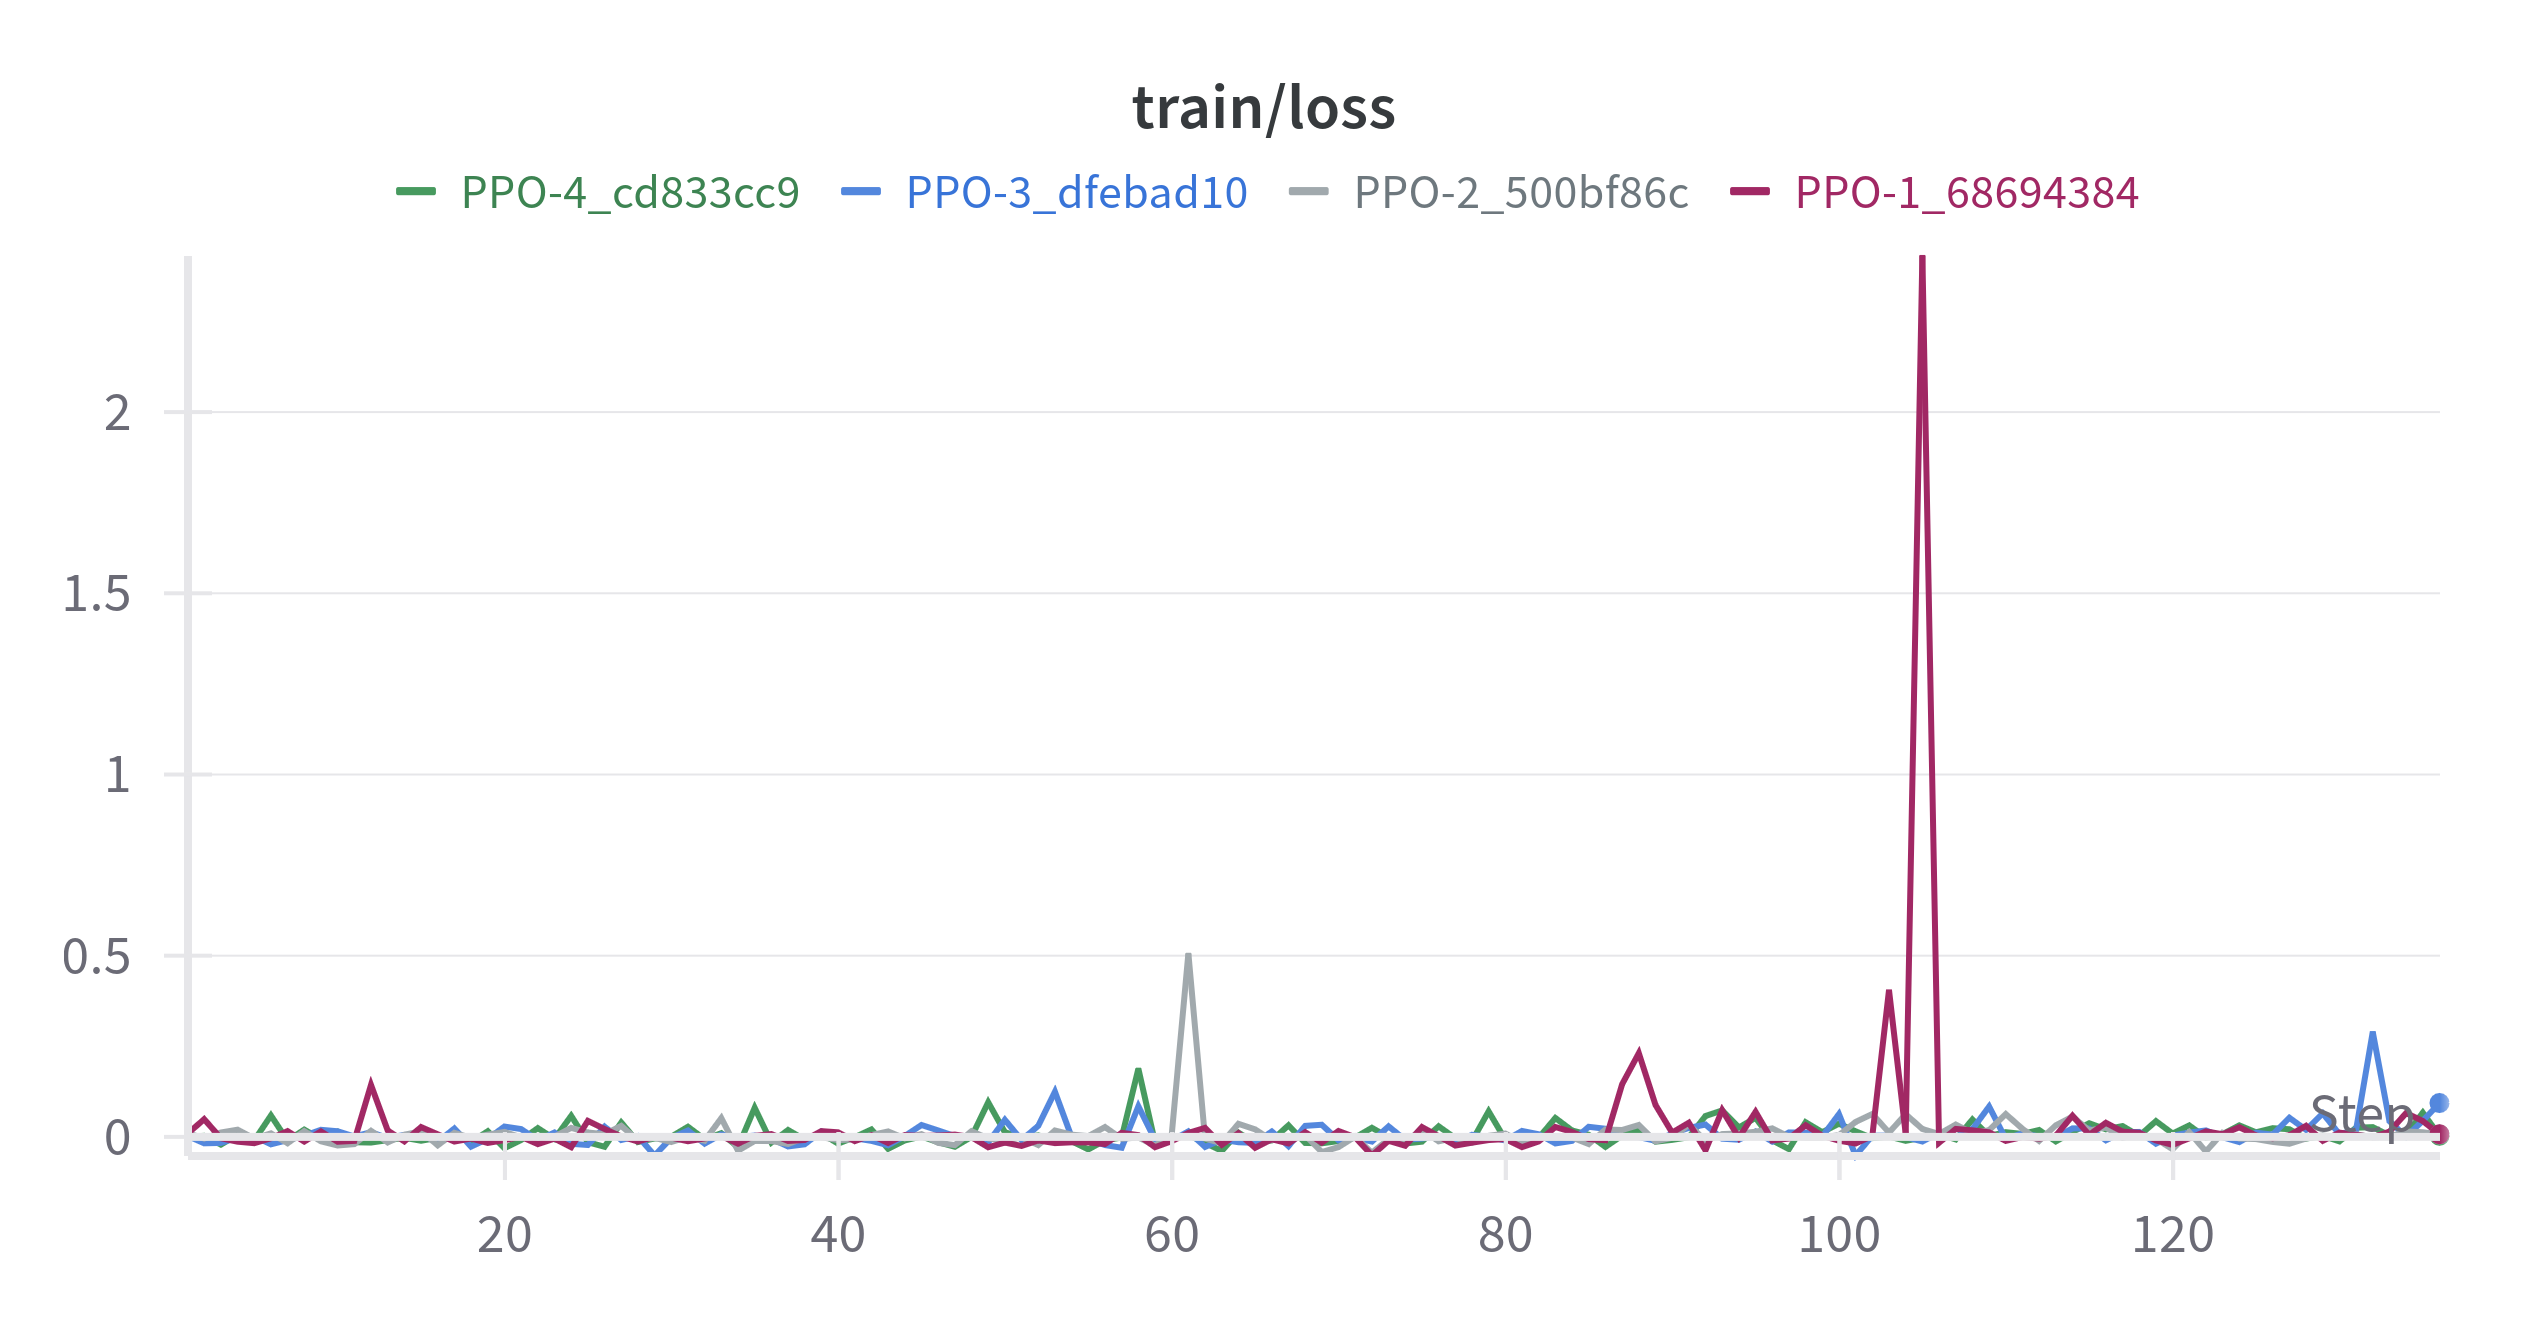
\includegraphics[width=0.8\textwidth]{figures/PPO_loss.png}
    \caption{Loss of All PPO Agents}
    \label{fig:agent_eval_all_ppo_loss}
\end{figure}

The figure above shows the training loss of each agent and shows that all 4 agents had consistently low loss values throughout the training with the exception of PPO agent 1, which had a large spike in loss at episode 100. Despite the spike in loss, the agent was able to recover and maintain a low loss value. However, the graph does not provide enough information to conclude the best performing agent, only that agent 1 experienced a large unexplanable spike in expected to experienced outcome. 

\begin{figure}[H]
    \centering
    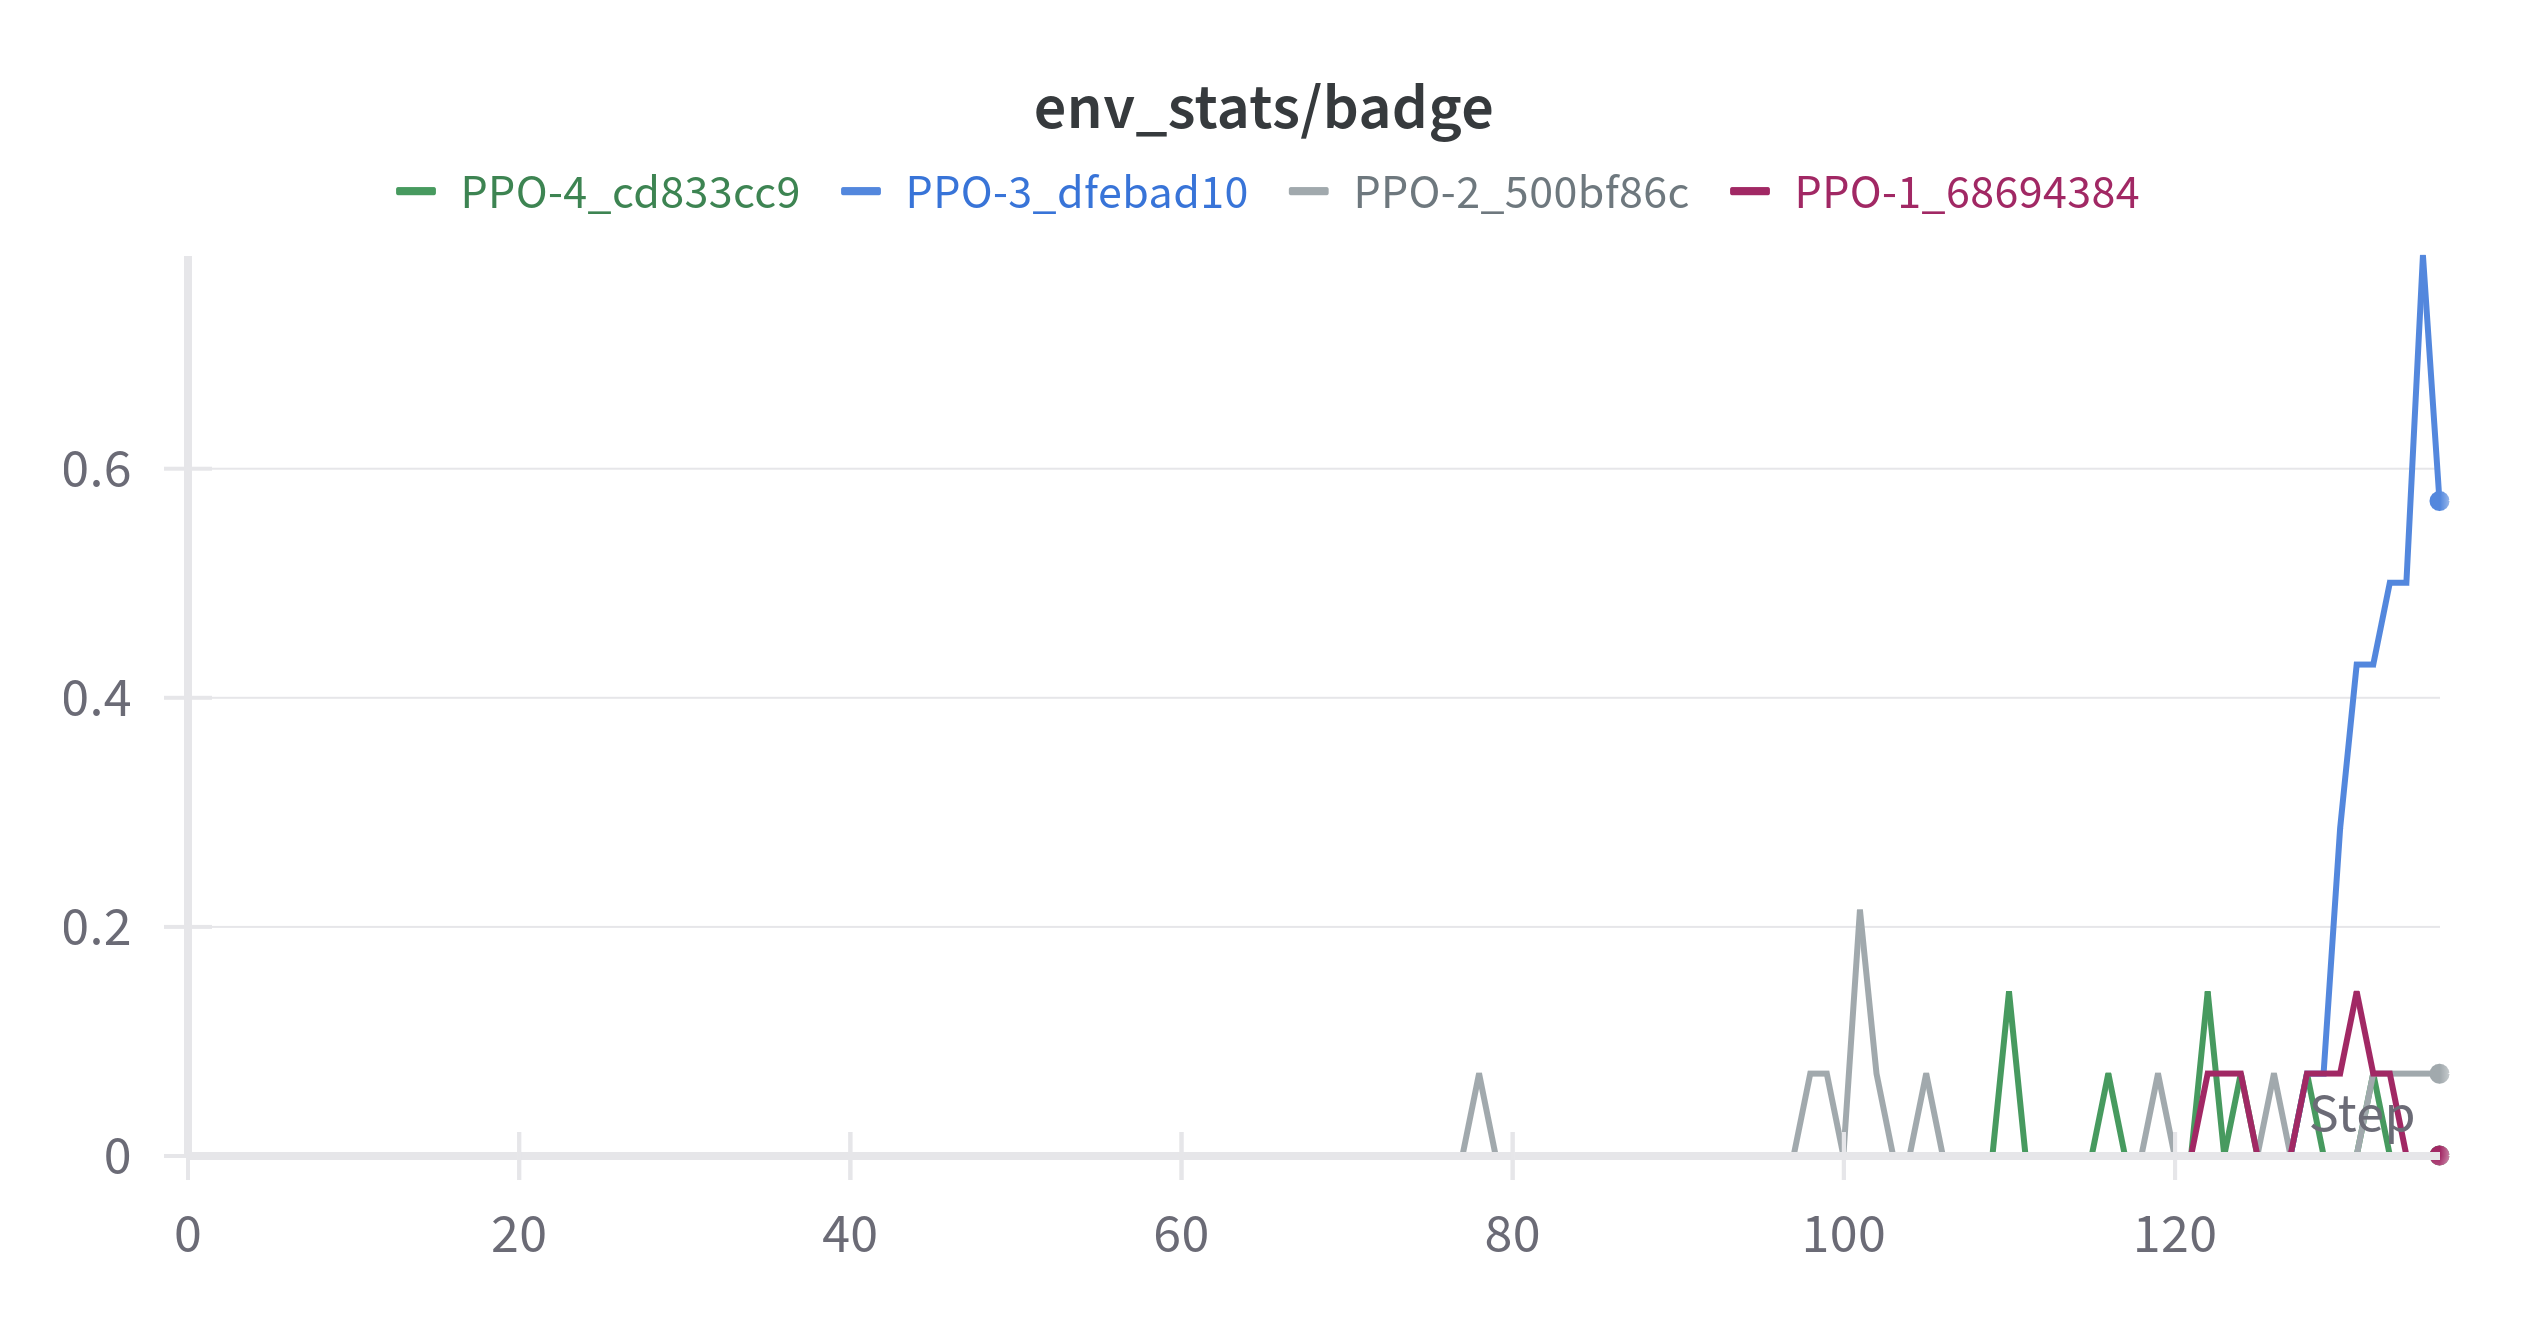
\includegraphics[width=0.8\textwidth]{figures/PPO_Badge.png}
    \caption{Badge Count of All PPO Agents}
    \label{fig:agent_eval_all_ppo_badge}
\end{figure}

To come to a conclusion as to which PPO agent is the best performing agent, figure \ref{fig:agent_eval_all_ppo_badge} showing the badge count of each agent will be used to determine which agent was able to complete the objective of this research the best by collecting the first gym badge the most consistently. The graph shows that all 4 agents were able to explore the environment enough to collect the first badge, however, PPO agent 2 was the agent to collect the first badge the earliest during training at episode 76. This is interesting as around the same episode, PPO agent 4 had a higher total\_reward than PPO agent 2. This suggests that the environment was explored differently by each agent and that the environment's reward function was not able to effectively guide the agent to reach the goal of collecting the first gym badge. Another interesting piece of information the graph confirms, is that agent 1 is the worst performing agent, as it was the second slowest agent to have one of the 10 instances collect the first gym, but also the agent with the least amount of consistency of instance of agents collecting the first gym badge. 

The most striking piece of information from the graph shows that agent 3 was the last to collect the first gym badge, but was the agent with the most consistent amount of instances to collect the first gym badge. With a peak of 80\% of the instances collecting the first gym badge by the end of training. This confirms that agent 3 is the best performing agent out of the 4 PPO agents.

\subsection{Algorithm Comparison}

The best performing agent from each algorithm will be compared to each other to determine which agent was able to balance out battling and navigation the best. The best performing agent from each algorithm was DQN agent 3, QR-DQN agent 1 and PPO agent 3. The performance of each agent will be compared through the use of comparing the total reward, loss, and badge count of each agent to determine their potential to complete the entire environment and how well they are able to achieve the objectives of this research within the training time frame of 40 million steps. 

One issue that arose while comparing the agents was that the agents were trained for different number of total episodes. Despite the total amount of timesteps being consistent betwewen all trained agents, the total amount of episodes was different because each algorithm had inconsistent number of instances of the environment being trained at the same time. This is because each algorithm took different amounts of RAM to train. Therefore, the graphs below will show the total timesteps taken on the x-axis instead of the total episodes. Next time, the number of environment instances and episodes will be kept consistent for further fairer testing. 

\begin{figure}[H]
    \centering
    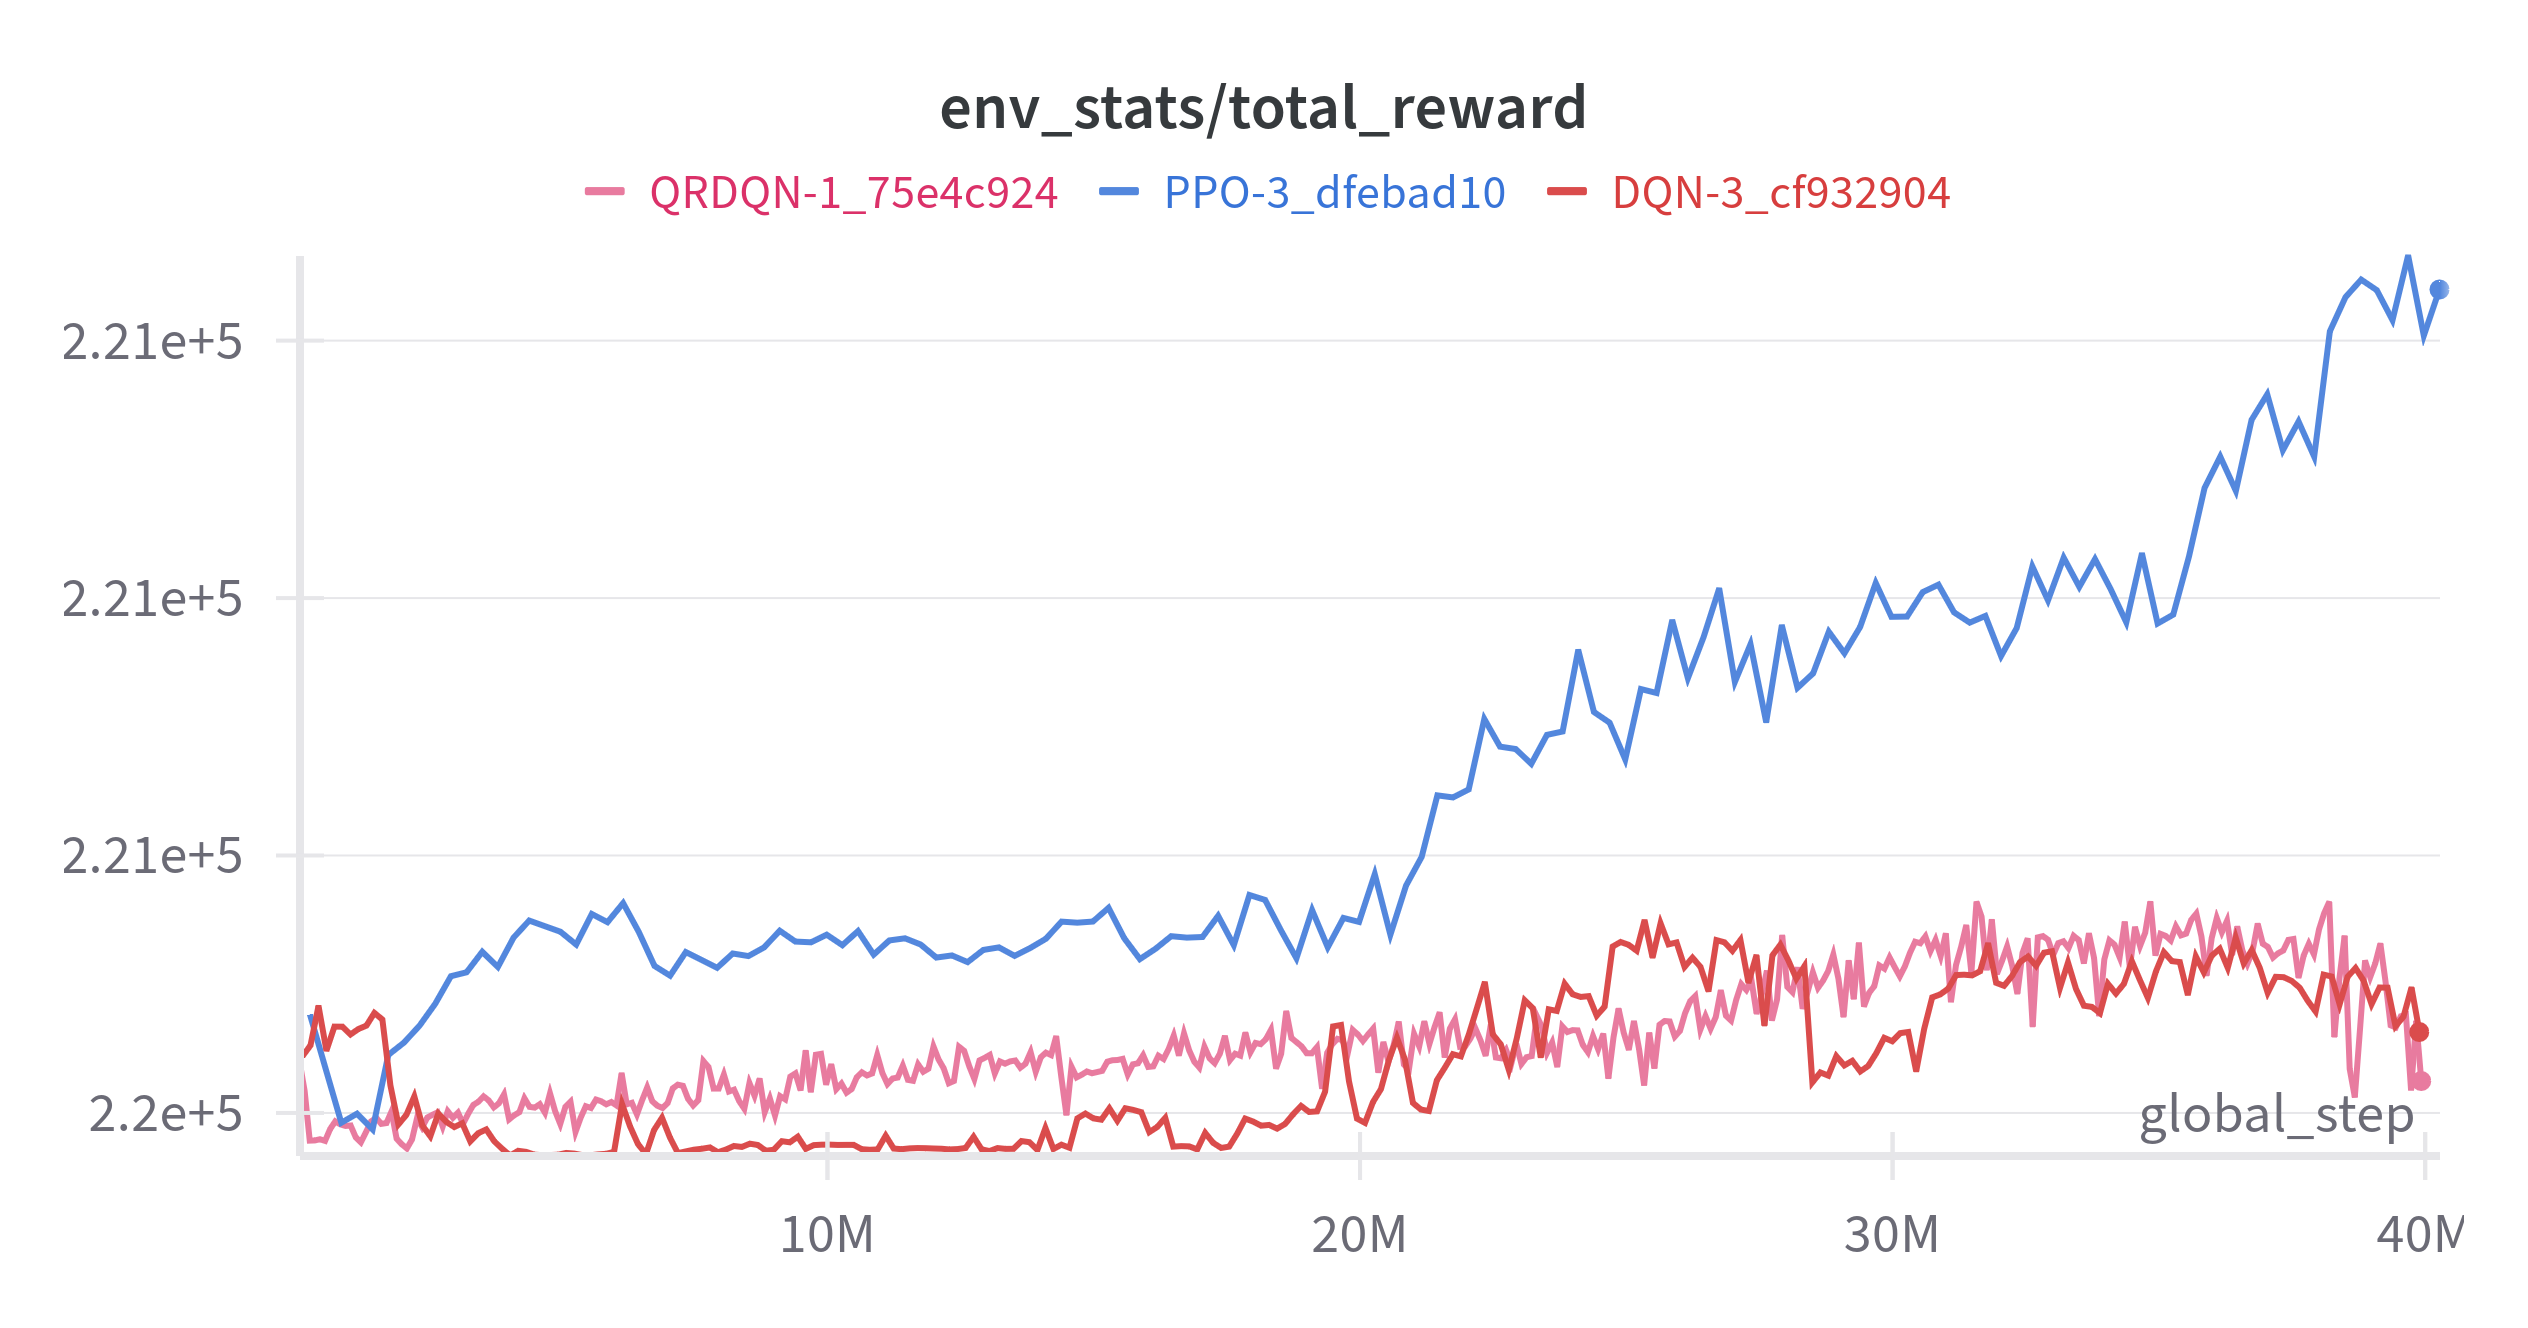
\includegraphics[width=0.8\textwidth]{figures/all_step_total_reward.png}
    \caption{}
    \label{fig:agent_eval_all_reward}
\end{figure}

Figure \ref{fig:agent_eval_all_reward} shows the total\_reward against total timesteps shows very evidently that PPO out performed DQN and QRDQN since the start. PPO was able to reach a higher amount of total reward within the first million timesteps compared to DQN and QRDQN. However, all 3 agents had similar rates of growth between 1 million and 20 million timesteps, which is suggested by the slopes of the agents being very similar. PPO showed a large spike in performance at around 20 million timesteps, which suggests that the agent was able to surpass a region of the environment which allowed for more reward to be gained. DQN and QRDQN comparitively did not show any signs of a spike in performance, which suggests that the agents were not able to reach the same region of the environment that PPO was able to reach. This is evident on figure \ref{fig:agent_eval_all_badge} below, showing the number of badges collected by each agent.

\begin{figure}[H]
    \centering
    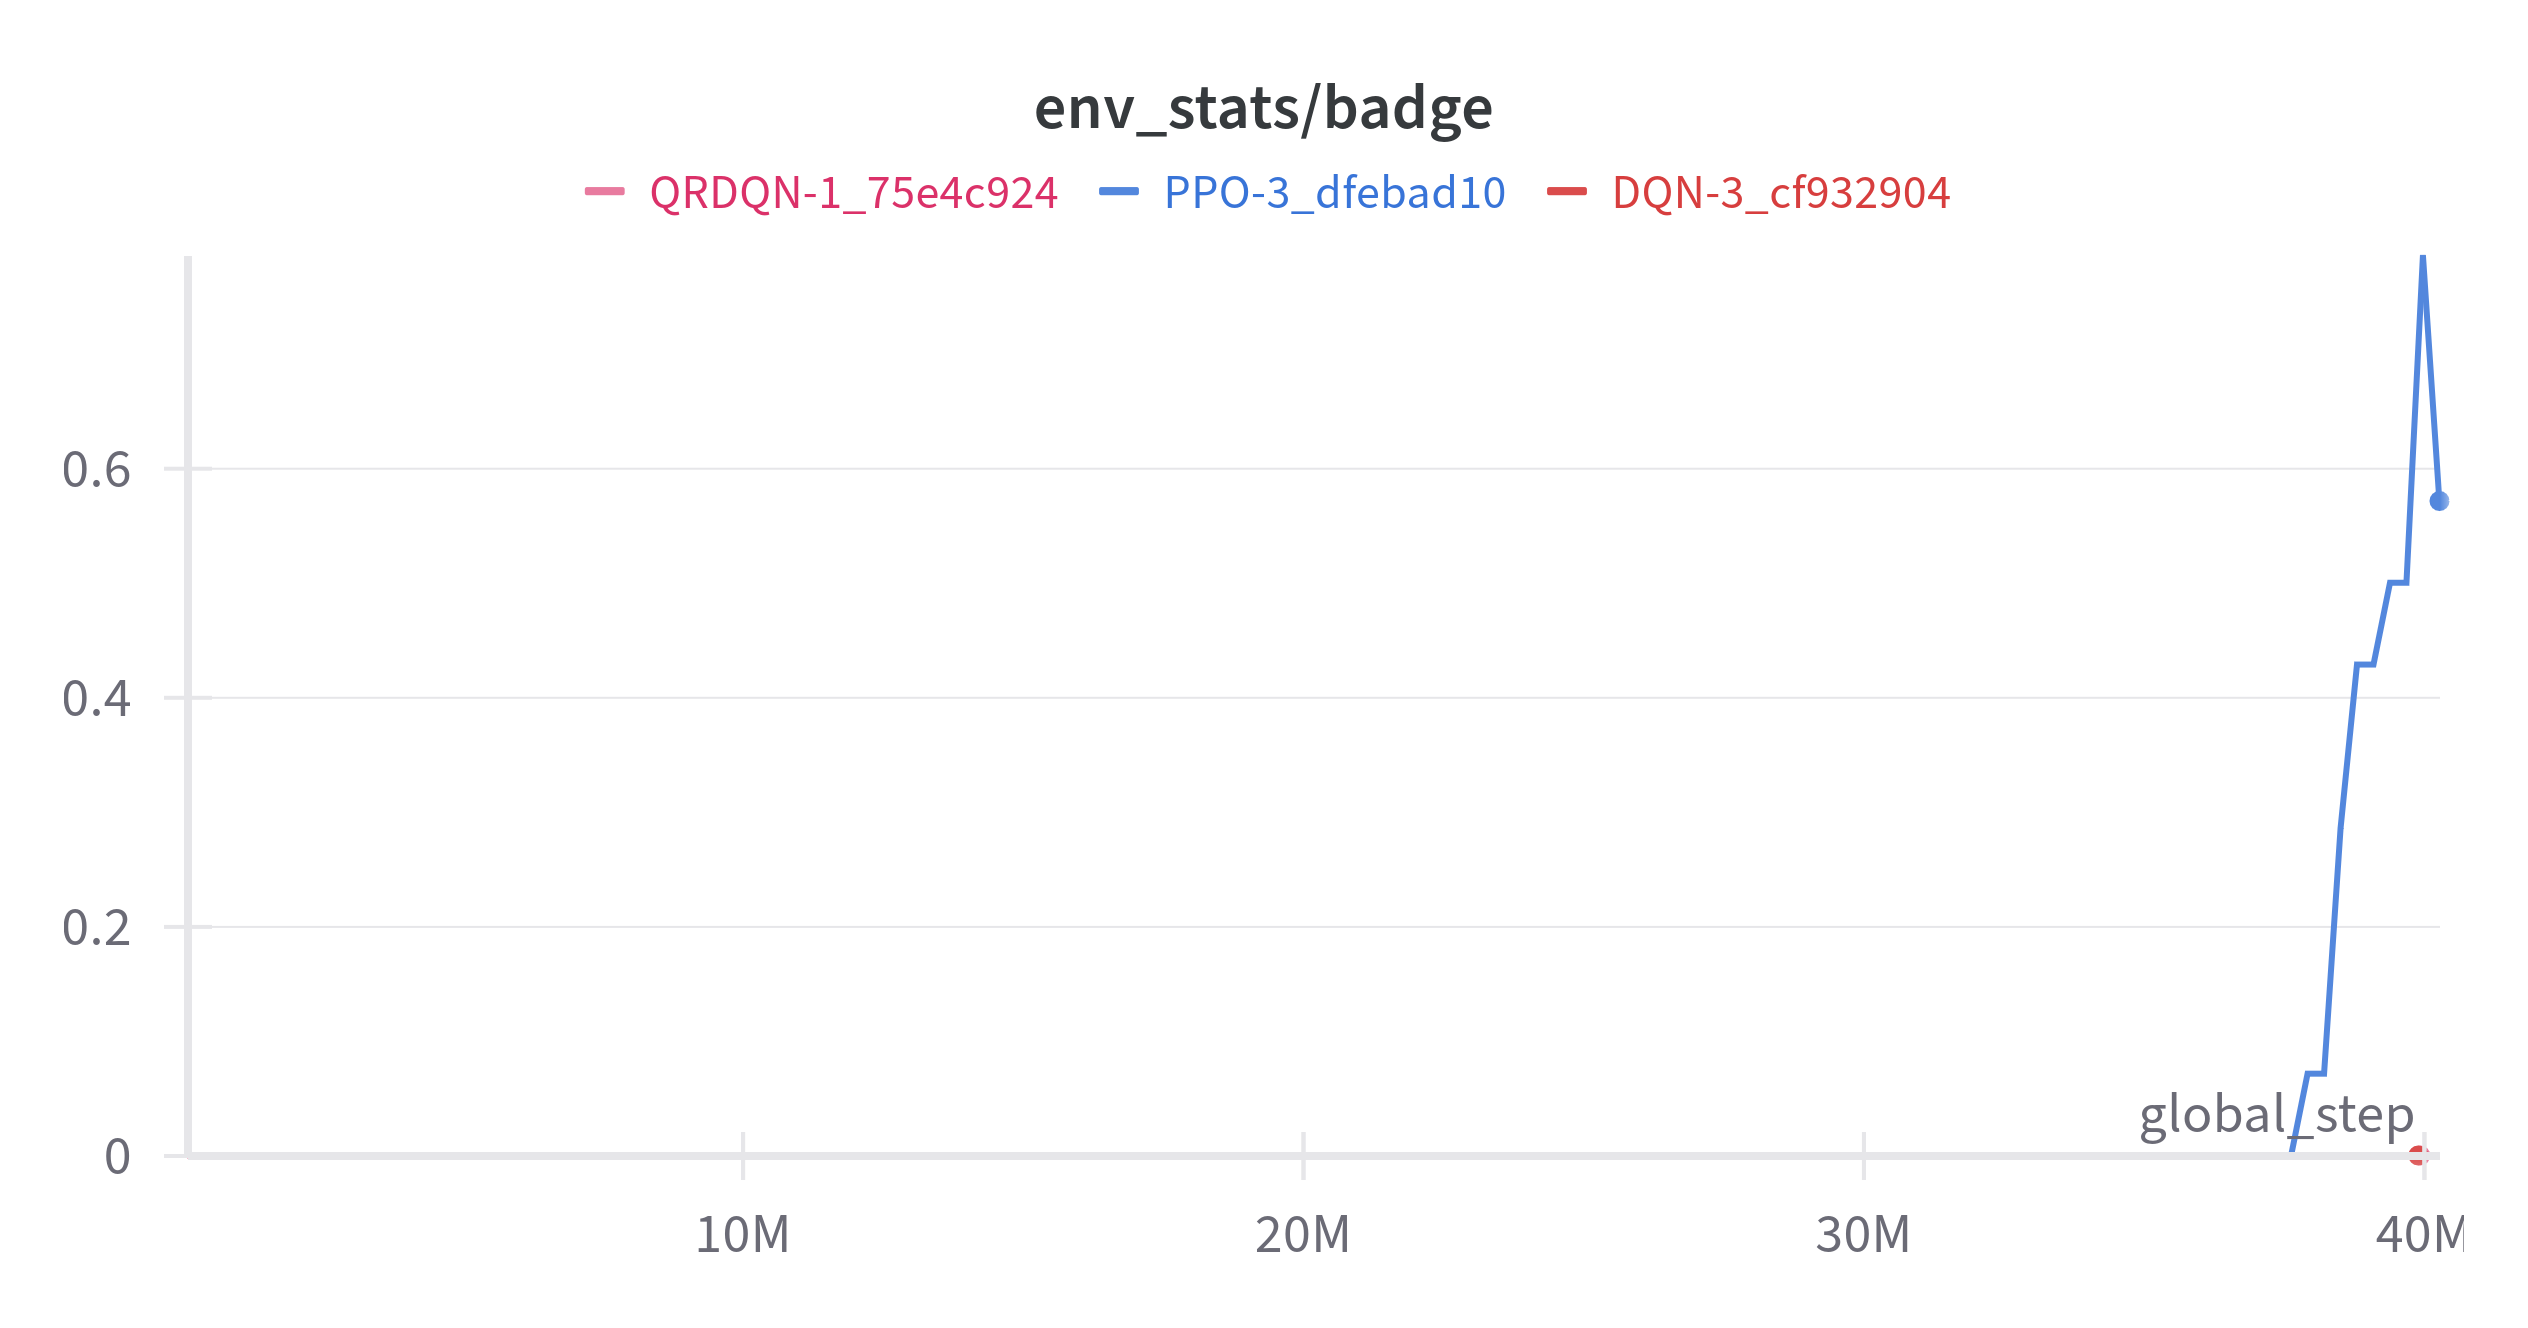
\includegraphics[width=0.8\textwidth]{figures/all_step_badge.png}
    \caption{}
    \label{fig:agent_eval_all_badge}
\end{figure}

This next graph shows the badge count of each agent against total timesteps. The graph shows that PPO was able to collect the first gym badge, where as DQN and QRDQN was never able to find the first gym badge. This suggests that PPO was able to explore the environment and overcome the challenges that DQN and QRDQN were not able to overcome, which is why PPO was the only agent able to collect the first gym badge. 

\begin{figure}[H]
    \centering
    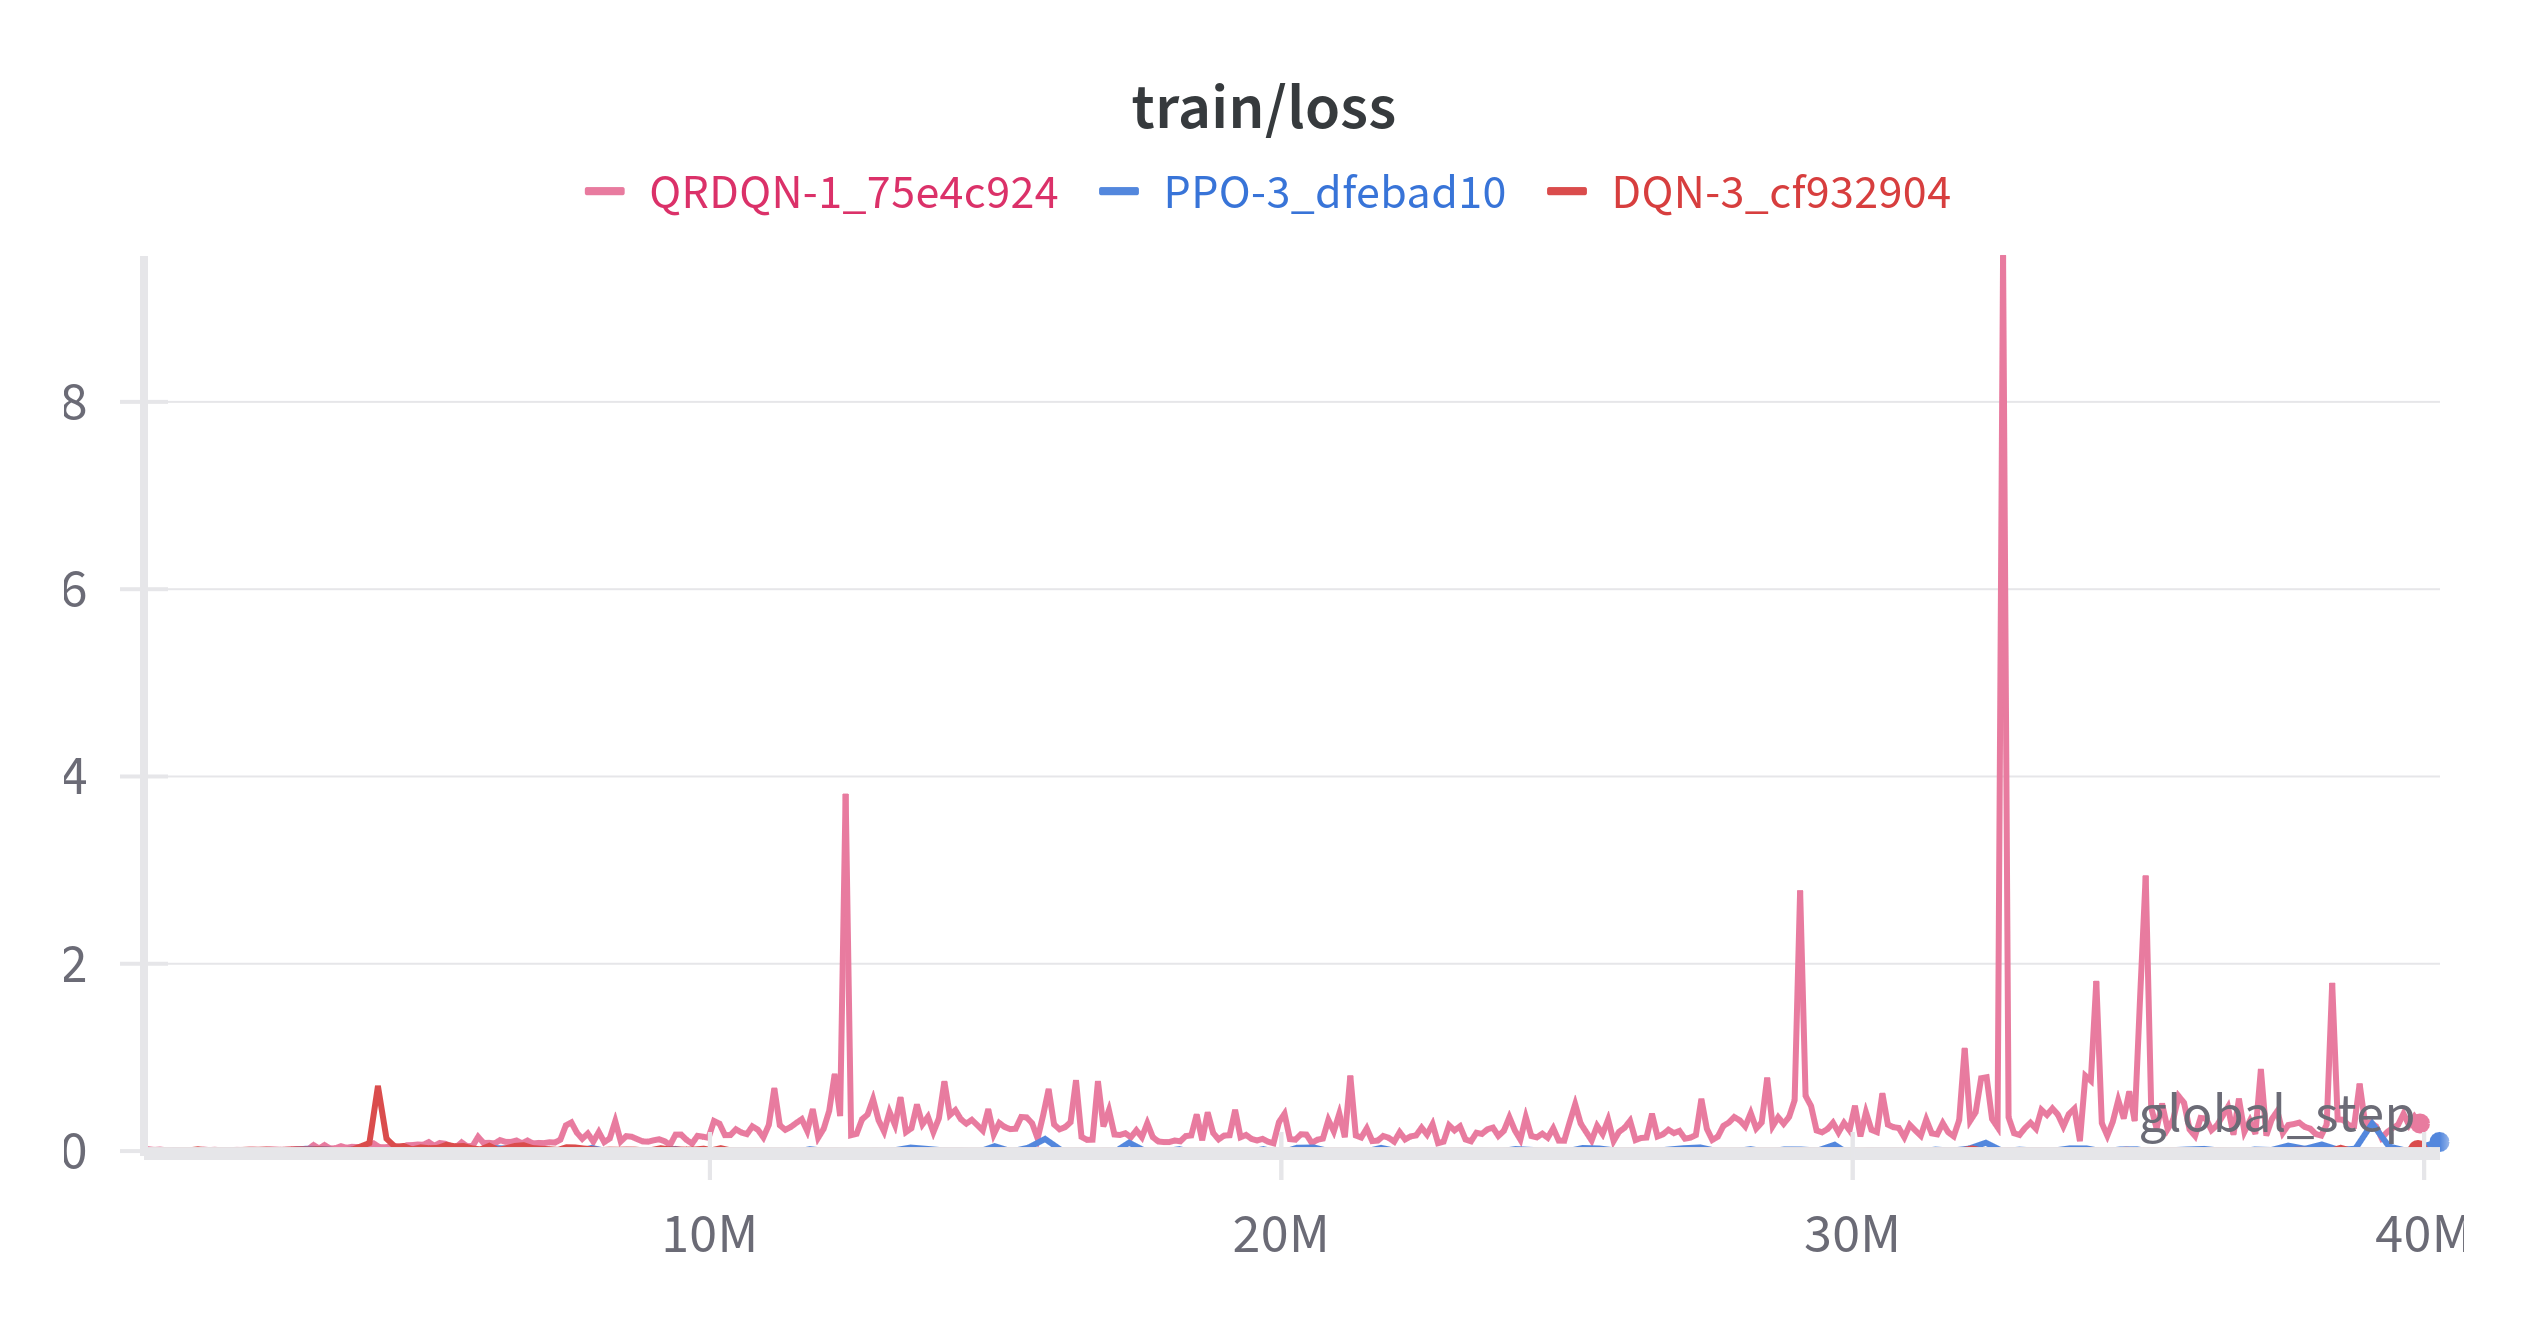
\includegraphics[width=0.8\textwidth]{figures/all_step_loss.png}
    \caption{}
    \label{fig:agent_eval_all_loss}
\end{figure}

Figure \ref{fig:agent_eval_all_loss} shows the loss of each agent against total timesteps. The graph very evidently highlights the turbulent nature of QRDQN training, as the agent had countless spikes of differing sizes. Where as DQN and PPO had very consistent low loss values throughout the training. This suggests that QRDQN had a very inconsistent training process and was not able to effectively learn what to expect within the environment compared to the actual outcome of the environment. It can be argued that the inconsistent training process is due to the low amount of reward achieved by QRDQN, which suggests that it was consistently exploring. However, the DQN agent had very similar levels of total reward to QRDQN and had a very consistent and low loss value while training. 

\subsection{Algorithm Comparison Conclusion}

In conclusion, it is evident that the PPO agent was the best performing agent out of the 3 agents. This is evident by the agents higher total reward, the only algorithm able to collect the first gym badge and the consistent low loss value throughout the training. This suggests that value based policies such as DQN and QRDQN are not as effective as policy based policies such as PPO when training agents to explore and exploit the environment. It is possible that the stochastic nature and massive search space of this environment makes it difficult for value based policies to learn the environment effectively. On the other hand, the reward function values to scale the amount of reward for exploration and battling were fine tuned to the PPO agent, which could have been the reason for the PPO agent outperforming the other agents. However, the complexity of the environment and the stochastic nature of the environment made it very difficult to determine the best reward function values to scale the amount of reward for exploration and battling without the use of a hyperparameter search and algorithms such as PPO. 

Despite the total reward performance of DQN and QRDQN being similar, the loss value of the DQN agent were better than QRDQN because of its stable performance throughout all 40 million timesteps. This suggests that DQN was able to learn the environment more effectively than QRDQN because of its ability to make consistent reward expectation throughout training.
